\section{Introduction}
The increasing penetration of the mobile devices, such as tablets and smart phones is generating a huge number of data traffic, especially video traffic over mobile networks \cite{ericsson,cisco_forecast}. In this context, it is common to have a huge number of devices associated with the LMA in a PMIPv6 domain, thus, easily making the LMA a bottleneck and single point of failure. Consequently, the quality of the ongoing sessions could be degraded (e.g., longer queuing delay, and increased packet loss). In this context, mobile network operators may need to deploy multiple LMAs in a large PMIPv6 domain, so that the traffic can be distributed among the LMAs \cite{PMIPv6}. Yet, it is highly possible that some LMAs become overloaded while others are underutilized. Consequently, load balancing (LB) among the LMAs is needed.

From the fact that multicast is expected to be widely deployed in the near future to deal with a huge demand of multimedia traffic, as well as the mobile video content typically has much higher bit rates than the other content types, the multicast service should play a crucial factor in putting load on the LMA. However, its role has been neglected in all existing LB proposals. Therefore, the consideration of multicast in the existing LB mechanisms can lead to several issues from both LB (efficiency degradation) and multicast service perspective (e.g., tunnel convergence problem and service disruption). 

For these reasons, a LB mechanism which takes the multicast service into account is needed. In this chapter, we will introduce such LB mechanism, the so-called multicast-based mechanism. The key idea is that by separating the multicast LB from the unicast LB, the proposed solution helps better distribute the load among the LMAs in runtime, thus, improving the efficiency of resource utilization. In details, when an LMA is overloaded, a multicast session will be selected to move to a less loaded one. The LB will also be executed when a listener starts a new multicast session to select the appropriate LMA to serve this session. As a result, the proposed solution does not influence the ongoing unicast/multicast sessions (except the selected session with which the multicast service disruption, in most cases, satisfies the requirements for the real-time services \cite{interruption_requirements}). It is noted that this chapter mainly focuses on the multicast listener.  

The rest of this chapter is organized as follows. Section \ref{ch7:existing_solution} highlights the issues when considering multicast with the existing LB mechanisms. Section \ref{ch7:solution} introduces the multicast-based LB as well as the criteria for the LMA and multicast session selection. Section \ref{ch7:performance_analysis} presents the performance analysis regarding LMA load and multicast service disruption. Section \ref{c7:experiment} takes a look on the experiment testbed including the testbed description, the experiment scenarios and the collected results. Finally, Section \ref{ch7:conclusion} concludes this chapter.

\section{Multicast Consideration in the Existing LB Mechanisms}\label{ch7:existing_solution}
There are two main approaches for LB among LMAs in PMIPv6, namely, proactive-MN and reactive-MN. In the proactive-MN approach \cite{runtime_lma, lma_discovery}, the LB will be executed in the initial phase of an MN to select the least loaded LMA. This approach only takes the current load of the LMAs (neither unicast nor multicast service) into account. All mobility sessions of this MN then would be anchored at the assigned LMA during their lifetime in the domain. The main advantage of this approach is that it does not influence the ongoing sessions of the registered MNs. However, since it is executed in the initial phase of an MN, the varying session rate and data rate may cause the unfair load distribution among the LMAs. When an LMA is overloaded, it may drop the new sessions. It also causes several issues for the ongoing sessions such as service disruption and packet loss. 
\begin{figure}[h!] 
 \begin{center} 
 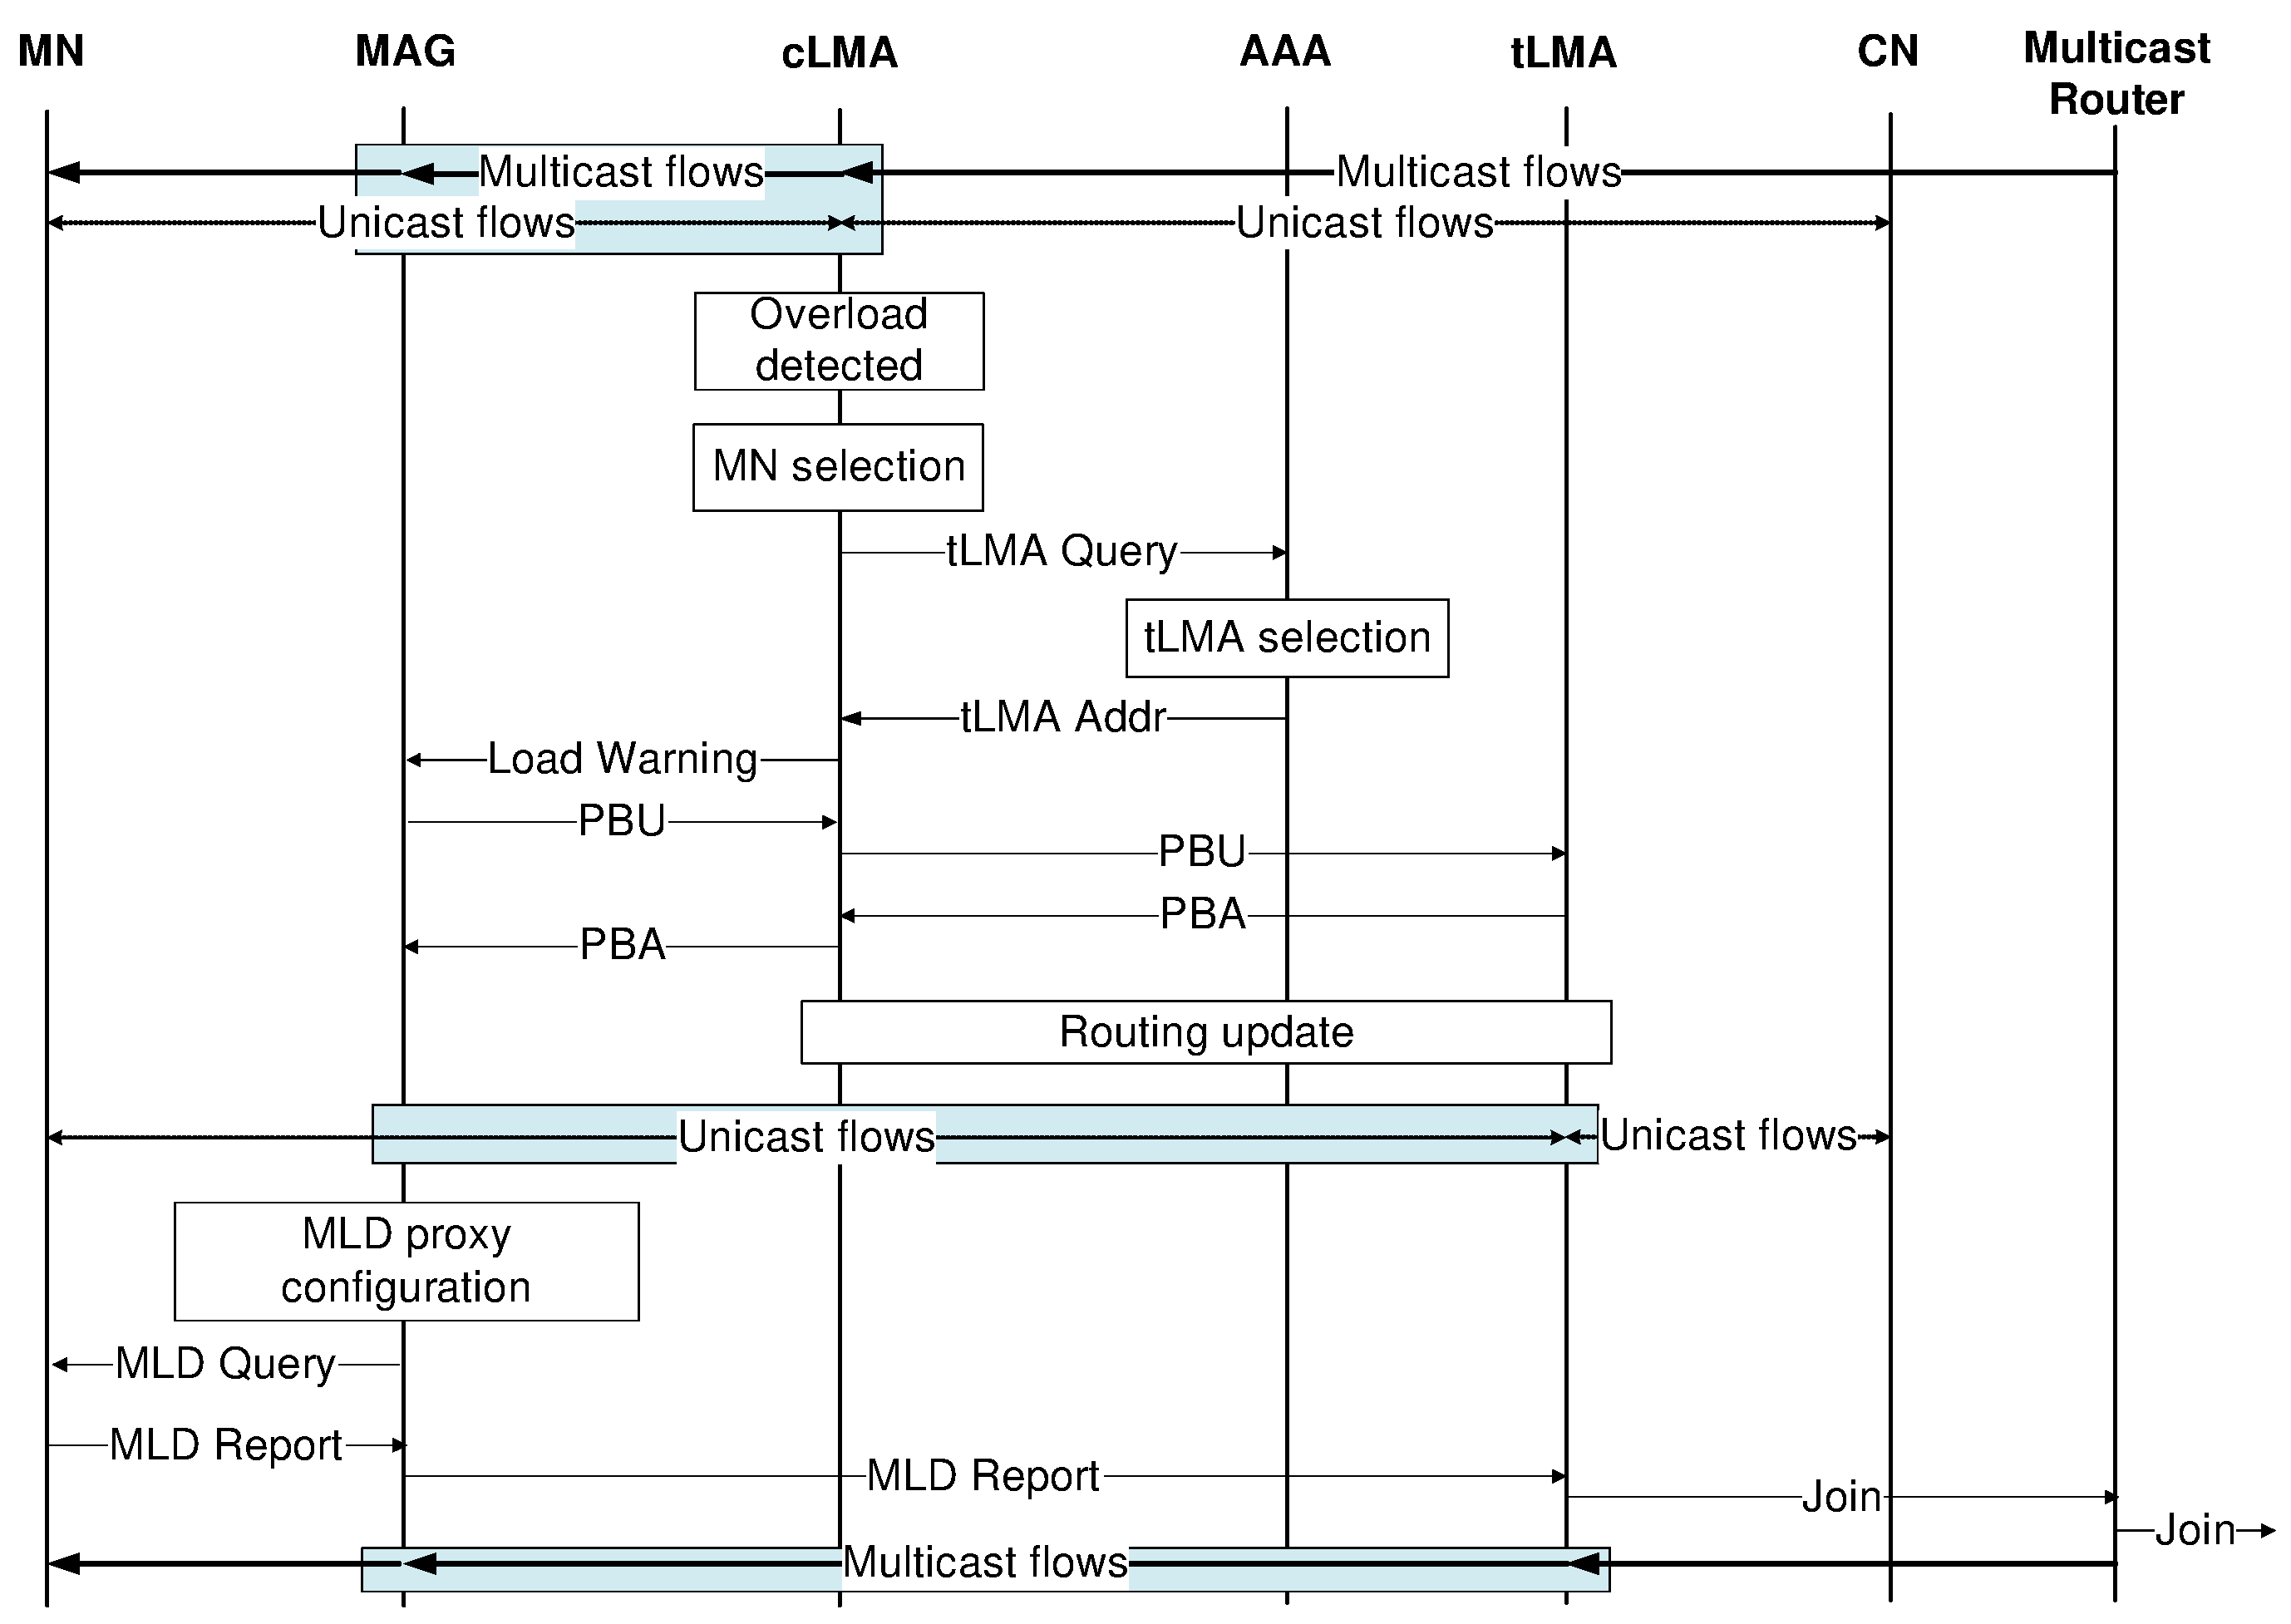
\includegraphics[width=0.70\textwidth]{./Part2/Chapter5/figures/reactive_MN_flow.eps} 
    \caption[Multicast considerations in the reactive-MN load balancing approach.]{Multicast considerations in the reactive-MN approach.}
     \label{fig:reactive_MN_flow}
  \end{center} 
\end{figure}

In the reactive-MN approach \cite{lb_lma,lb_mobility_session}, the LB will be triggered when the LMA load exceeds a specified threshold. The overloaded LMA will select one (or several) MN(s) to move to a less loaded LMA (called target LMA, or tLMA). The load information of all LMAs can be collected and managed at the authentication, authorization and accounting (AAA) server which then selects the tLMA among the LMAs in the domain. The PBU/PBA messages then are exchanged between the current LMA (cLMA) and the tLMA allowing the tLMA to serve as a new mobility anchor of the MN. This approach allows the network to adapt to the current situation. Thus, it may give a better performance e.g., distributing load among LMAs and increasing the reliability. Since the LMA plays the role of the mobility anchor for the MN, changing LMA during the mobility session could impact the selected MN’s ongoing sessions. For this reason, this change is not recommended by the IETF \cite{runtime_lma,lma_discovery}. In addition, the existing proposals only consider the ongoing sessions as the unicast ones. How the LB works with the multicast is still an open question.
 
To support multicast in a PMIPv6 domain, the multicast router (MR) and the MLD proxy function need to be deployed at the LMA and the MAG, respectively \cite{RFC_6224}. In the base solution, a listener always receives the multicast traffic from its LMA via the LMA-MAG tunnel. As stated earlier, several procedures need to be executed in order to allow the MAG to continue receiving the traffic (from the tLMA). As a result, it experiences a noticeable service disruption for the ongoing multicast channels. Additional mechanisms (e.g., MLD proxy peering function \cite{multicast_source}) are required to reduce the service disruption time. 

If there is more than one listener (including the selected one) associated with the cLMA and subscribing to the same multicast channel, the cLMA will continue forwarding this channel. Consequently, moving the MN cannot help significantly reduce the LMA load, especially when the load generated by this MN is mainly from this channel. The total load of all LMAs may also be increased since the tLMA may need to join the channel. In addition, as the LMA selection algorithm does not take multicast into account, the tLMA may not support the multicast capability. In other words, the multicast service cannot be guaranteed at the tLMA. Also, since many proxy instances are installed at MAG, it may cause the tunnel convergence problem.   

\section{Multicast-based Load Balancing Solution}\label{ch7:solution}
In this section, at first, some criteria to select the appropriate LMA and multicast session for the LB purpose will be discussed. Two different approaches of the multicast-based solution i.e., the proactive-multicast (or MAG-initiated) and the reactive-multicast (or LMA-initiated) approach are then considered. In the former case, LB will be invoked when an MN starts a new multicast session to select a suitable LMA to serve this session. In the latter case, LB will be executed when an LMA is overloaded by selecting a multicast session to move to the less loaded one. It can be done thanks to an extension to MLD proxy to support multiple upstream interfaces \cite{multiple_upstreams}. In this case, only one proxy instance is deployed at MAG with multiple upstream interfaces being configured towards different LMAs. As a result, the MN can receive the multicast traffic from a less loaded LMA, while obtaining the unicast traffic from its LMA. Further information can be found in \cite{Thinh_elsevier_LB, Thinh_ICNC}.
\paragraph{Target LMA Selection}
Target LMA selection is first based on the channel policy which is defined by the operators (if exist). Otherwise, the LMA selection relies on the following policies (from high to low priority):  i) The least loaded LMA among the (not overloaded) LMAs having the multicast forwarding state for this channel should be selected; and ii) The LMA with the lowest load in the domain should be selected. The selection policies come from the fact that if the channel is already available at the selected LMA (target LMA, or tLMA) with a negligible increase of load, the tLMA can forward this channel to the MAG \cite{developing_ip_multicast}. To do so, a new logical entity, the so-called load balancing controller (LBC), has been introduced. This entity collects and manages the load state information of all LMAs in the domain. It is also responsible for the LMA selection. 
Upon the location of the LBC, three different schemes can be considered as below:
\begin{itemize}
\item{Centralized LBC entity}: The functionality of the LBC is responsible by a central entity, called C-LBC. 
This entity is similar to the notion of rfLMA as described in \cite{runtime_lma}. The LMAs periodically report their current load to the C-LBC by using an extension to the PBA/PBU message with the load information \cite{runtime_lma}. The C-LBC can be co-located with the AAA server.
\item{Distributed LBC function on the LMAs}: The LBC function is executed in a distributed manner among the LMAs. Each LMA maintains a so-called Load Table which includes load information of all LMAs in the PMIPv6 domain. Each LMA periodically exchanges its load information with each other in the domain, for example, by setting a common multicast group for all LMAs.
\item{Distributed LBC function on the MAGs}: In this case, the load of all LMAs is collected and stored at the MAGs. The MAG can obtain the current load of the associated LMA by using an extension of PBU/PBA messages or an extension of the Heartbeat message with the load information \cite{lb-802.11}. 
\end{itemize}

Without loss of generality, this chapter only considers the first scheme. As all LMAs periodically report their workload to the C-LBC, the frequency of the workload report should be carefully examined as the trade-off between the precision of the load state and the signaling/processing overhead. One possible solution is that the LMA only reports its workload when its load exceeds/is lower than a certain load level. 

\paragraph{Multicast Session Selection}
The multicast session can be selected following some criteria: i) To reduce the potential impact on the ongoing session, the real-time and delay-sensitive session should not be selected. However, if all sessions are the real-time and delay-sensitive ones, the session with the highest data rate should be selected; and ii) The session requiring the highest data rate with the smallest number of subscribed listeners should be selected. It is noted that to better select LMA, the LMA selection algorithm should take the expected load of the selected multicast session into account.
%\vspace{-0.1in}
\subsection{Load Balancing in the Proactive-Multicast Approach}
\begin{figure}[h!] 
 \begin{center} 
 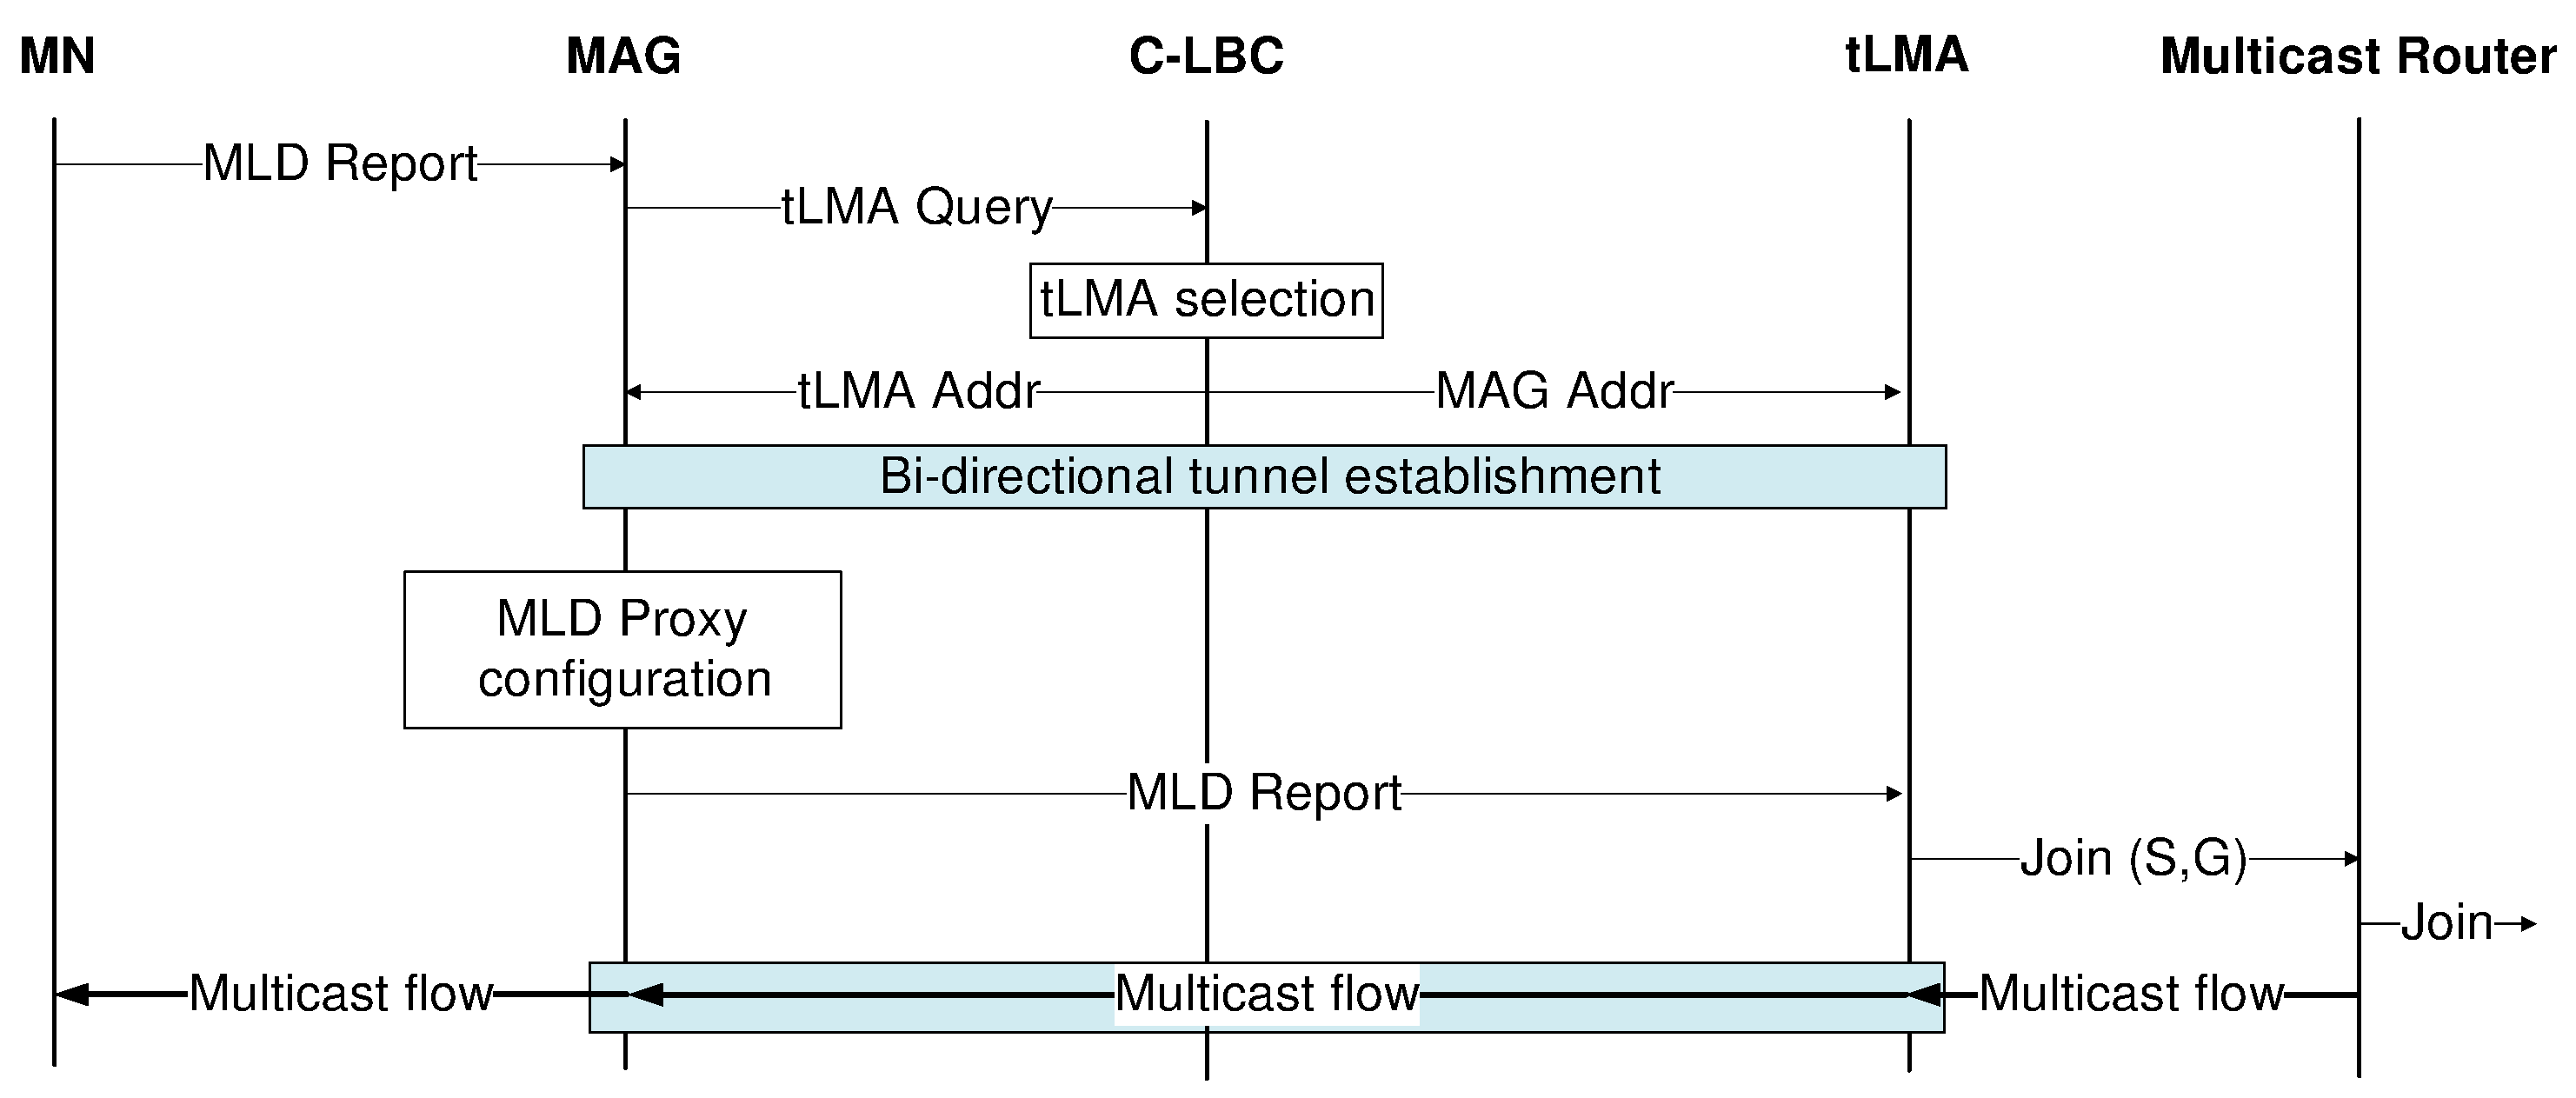
\includegraphics[width=0.65\textwidth]{./Part2/Chapter5/figures/c7_proactive_multicast.eps} 
    \caption[The proactive-multicast load balancing approach.]{Proactive-multicast approach.}
    \label{fig:proactive_multicast}
  \end{center} 
\end{figure}
The signaling procedure for the proactive-multicast (MAG-initiated) approach is illustrated in Fig.~\ref{fig:proactive_multicast}. When a registered MN wishes to subscribe to a multicast channel and this channel is available at the current MAG, the MAG will forward it directly to the MN. Otherwise, it will contact the C-LBC to get the address of an LMA (following the criteria as stated earlier), which can be served as the multicast anchor point for this session. After joining the channel via the tLMA, the MAG can receive the multicast packets and forwards them to the MN. Note that the communication between the MAG and the C-LBC can be done by extending the Remote Authentication Dial In User Service (RADIUS) protocol for PMIPv6 \cite{radius}.

\subsection{Load Balancing in the Reactive-Multicast Approach}
\begin{figure}[h!] 
 \begin{center} 
 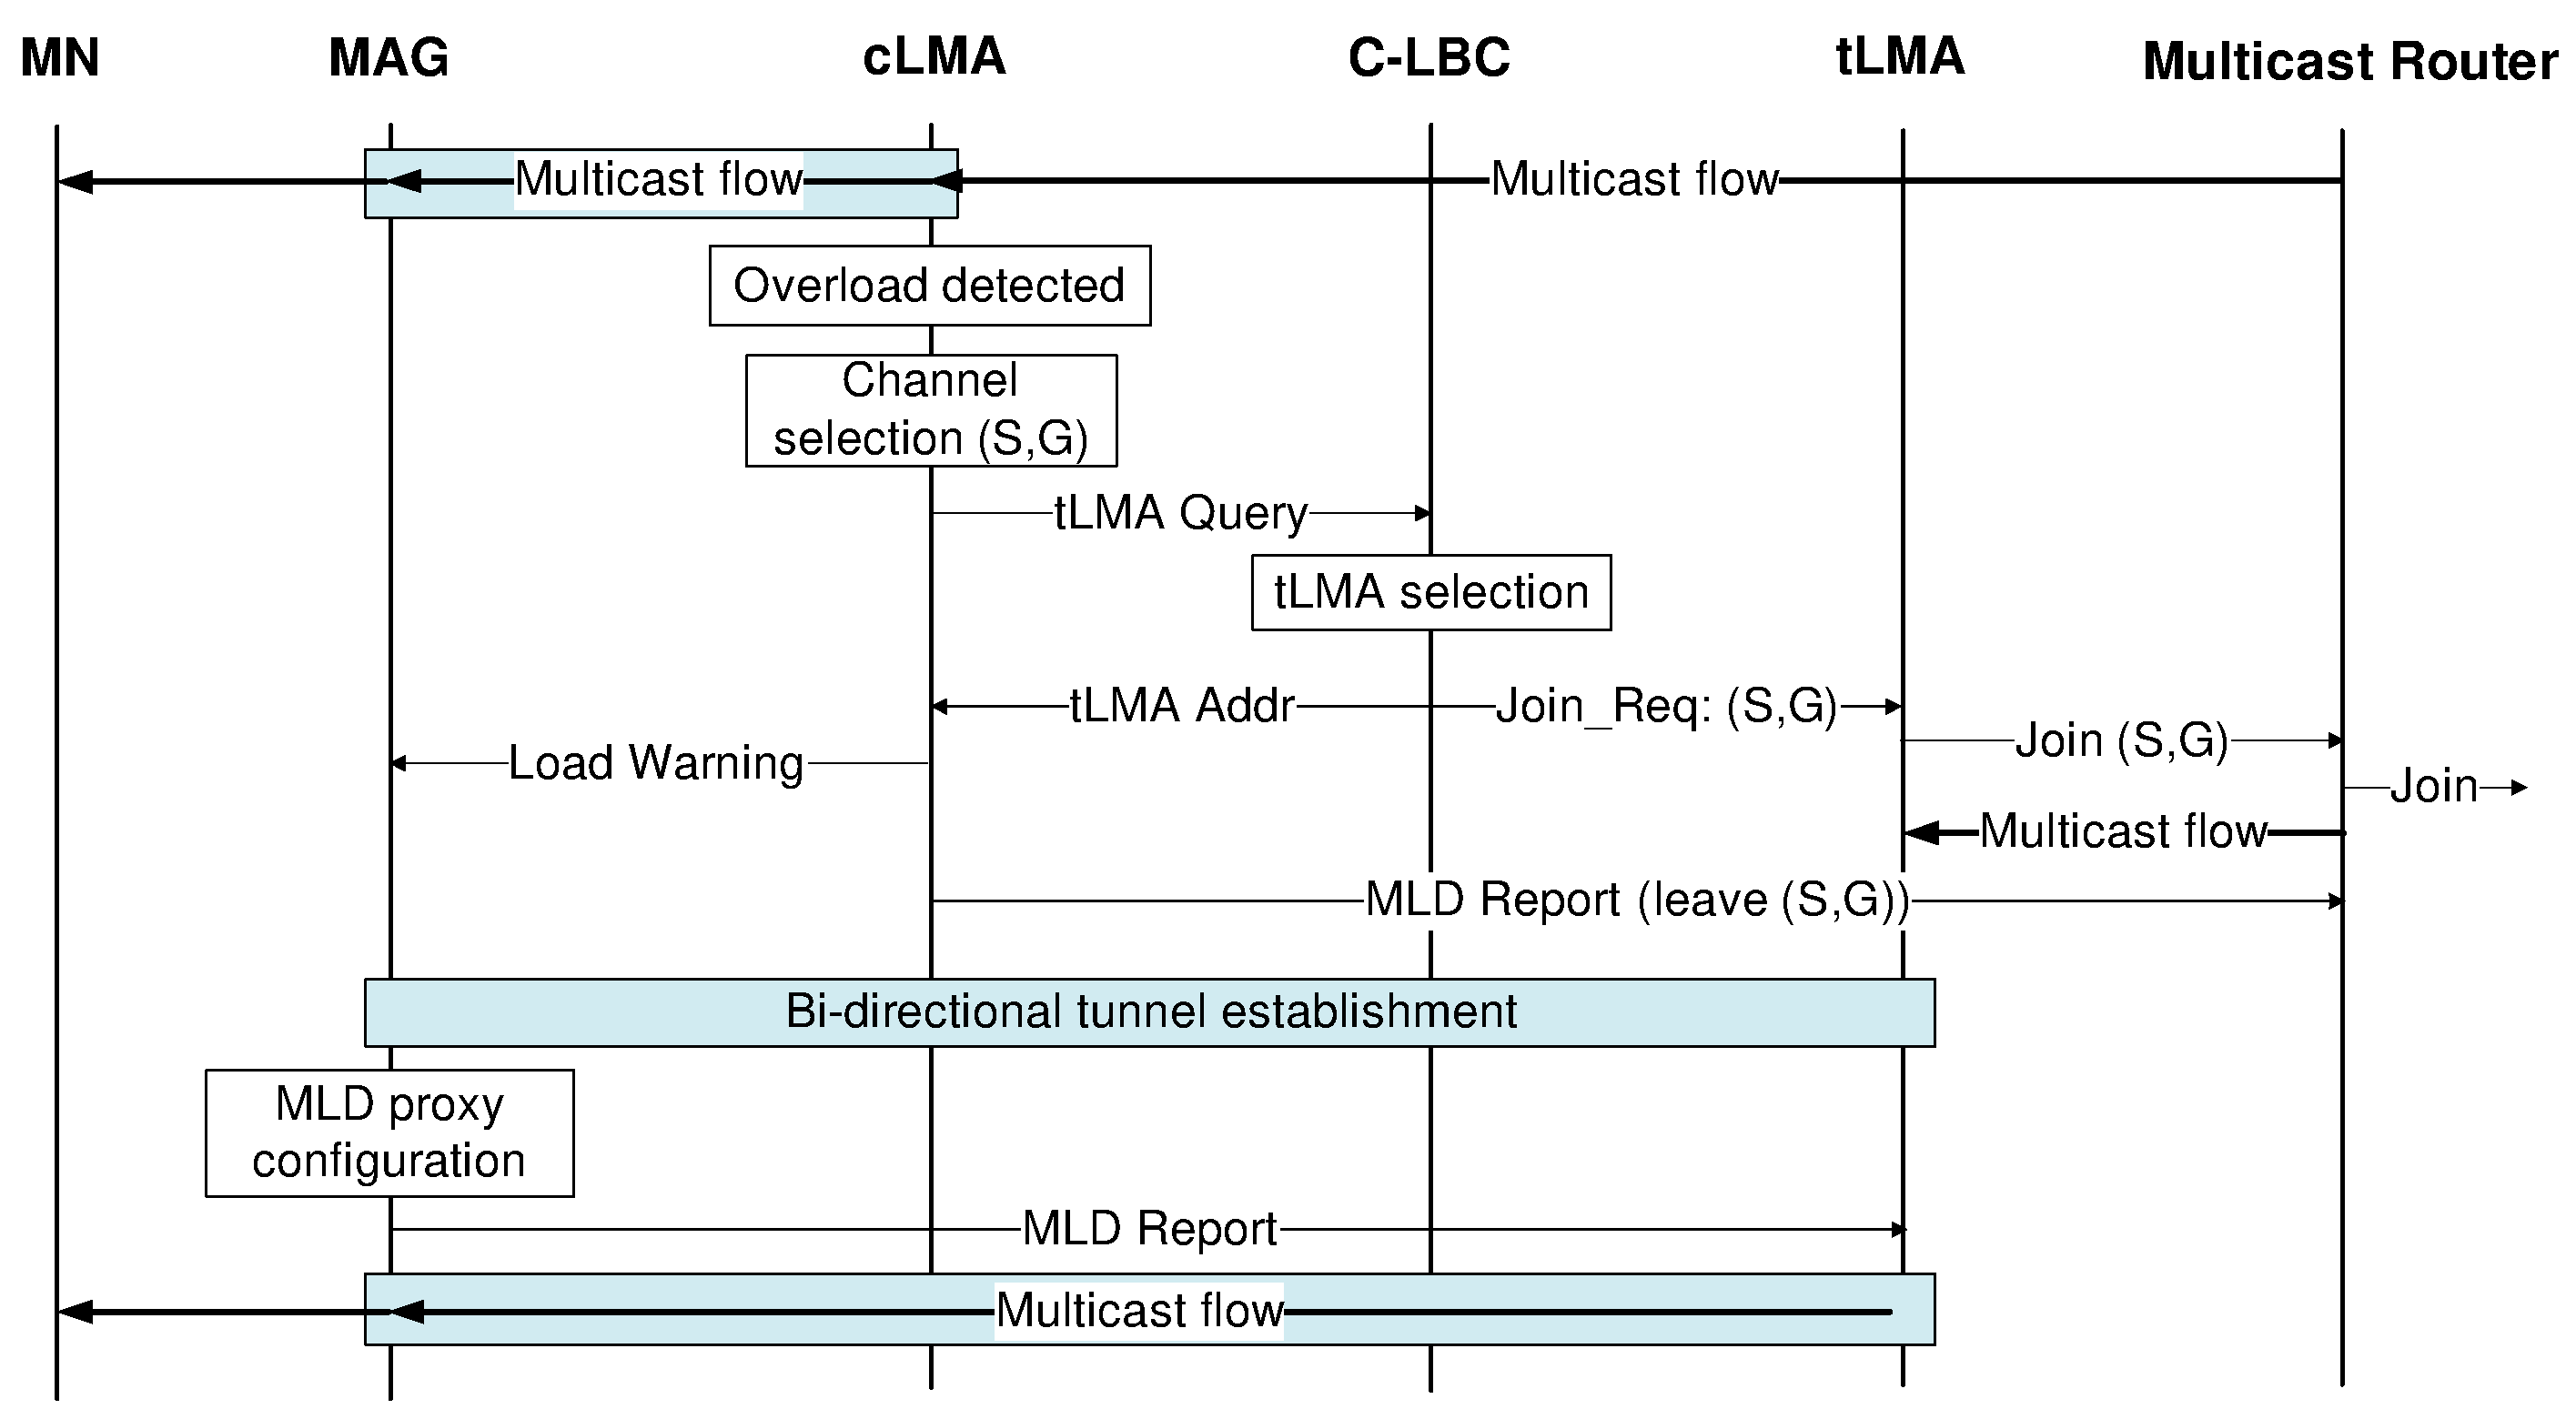
\includegraphics[width=0.70\textwidth]{./Part2/Chapter5/figures/reactive_multicast.eps} 
    \caption[The reactive-multicast load balancing approach.]{Reactive-multicast approach.}
        \label{fig:reactive_multicast}
  \end{center} 
\end{figure}

Fig.~\ref{fig:reactive_multicast} shows the signaling procedure for the reactive-multicast (LMA-initiated) approach. When an LMA (cLMA) is overloaded (its load exceeds a certain threshold), a multicast session will be selected to move from this LMA to a less loaded one (tLMA).
After obtaining the tLMA address from the C-LBC, the cLMA sends the tLMA's address and the selected multicast session information to all related MAGs via a load-warning message (e.g., using an extension to the Update Notification message (UNP) \cite{update_notification}). The C-LBC also requests the tLMA to join the channel in advance to reduce the multicast service disruption. The MAG then sends an MLD Report to the tLMA to join the channel. Afterwards, the MAG can receive the multicast packets from the tLMA instead from the cLMA. In the meantime, the cLMA can leave this channel in order to lower its load.
\subsection{Handover Consideration}
\begin{figure}[h!] 
 \begin{center} 
 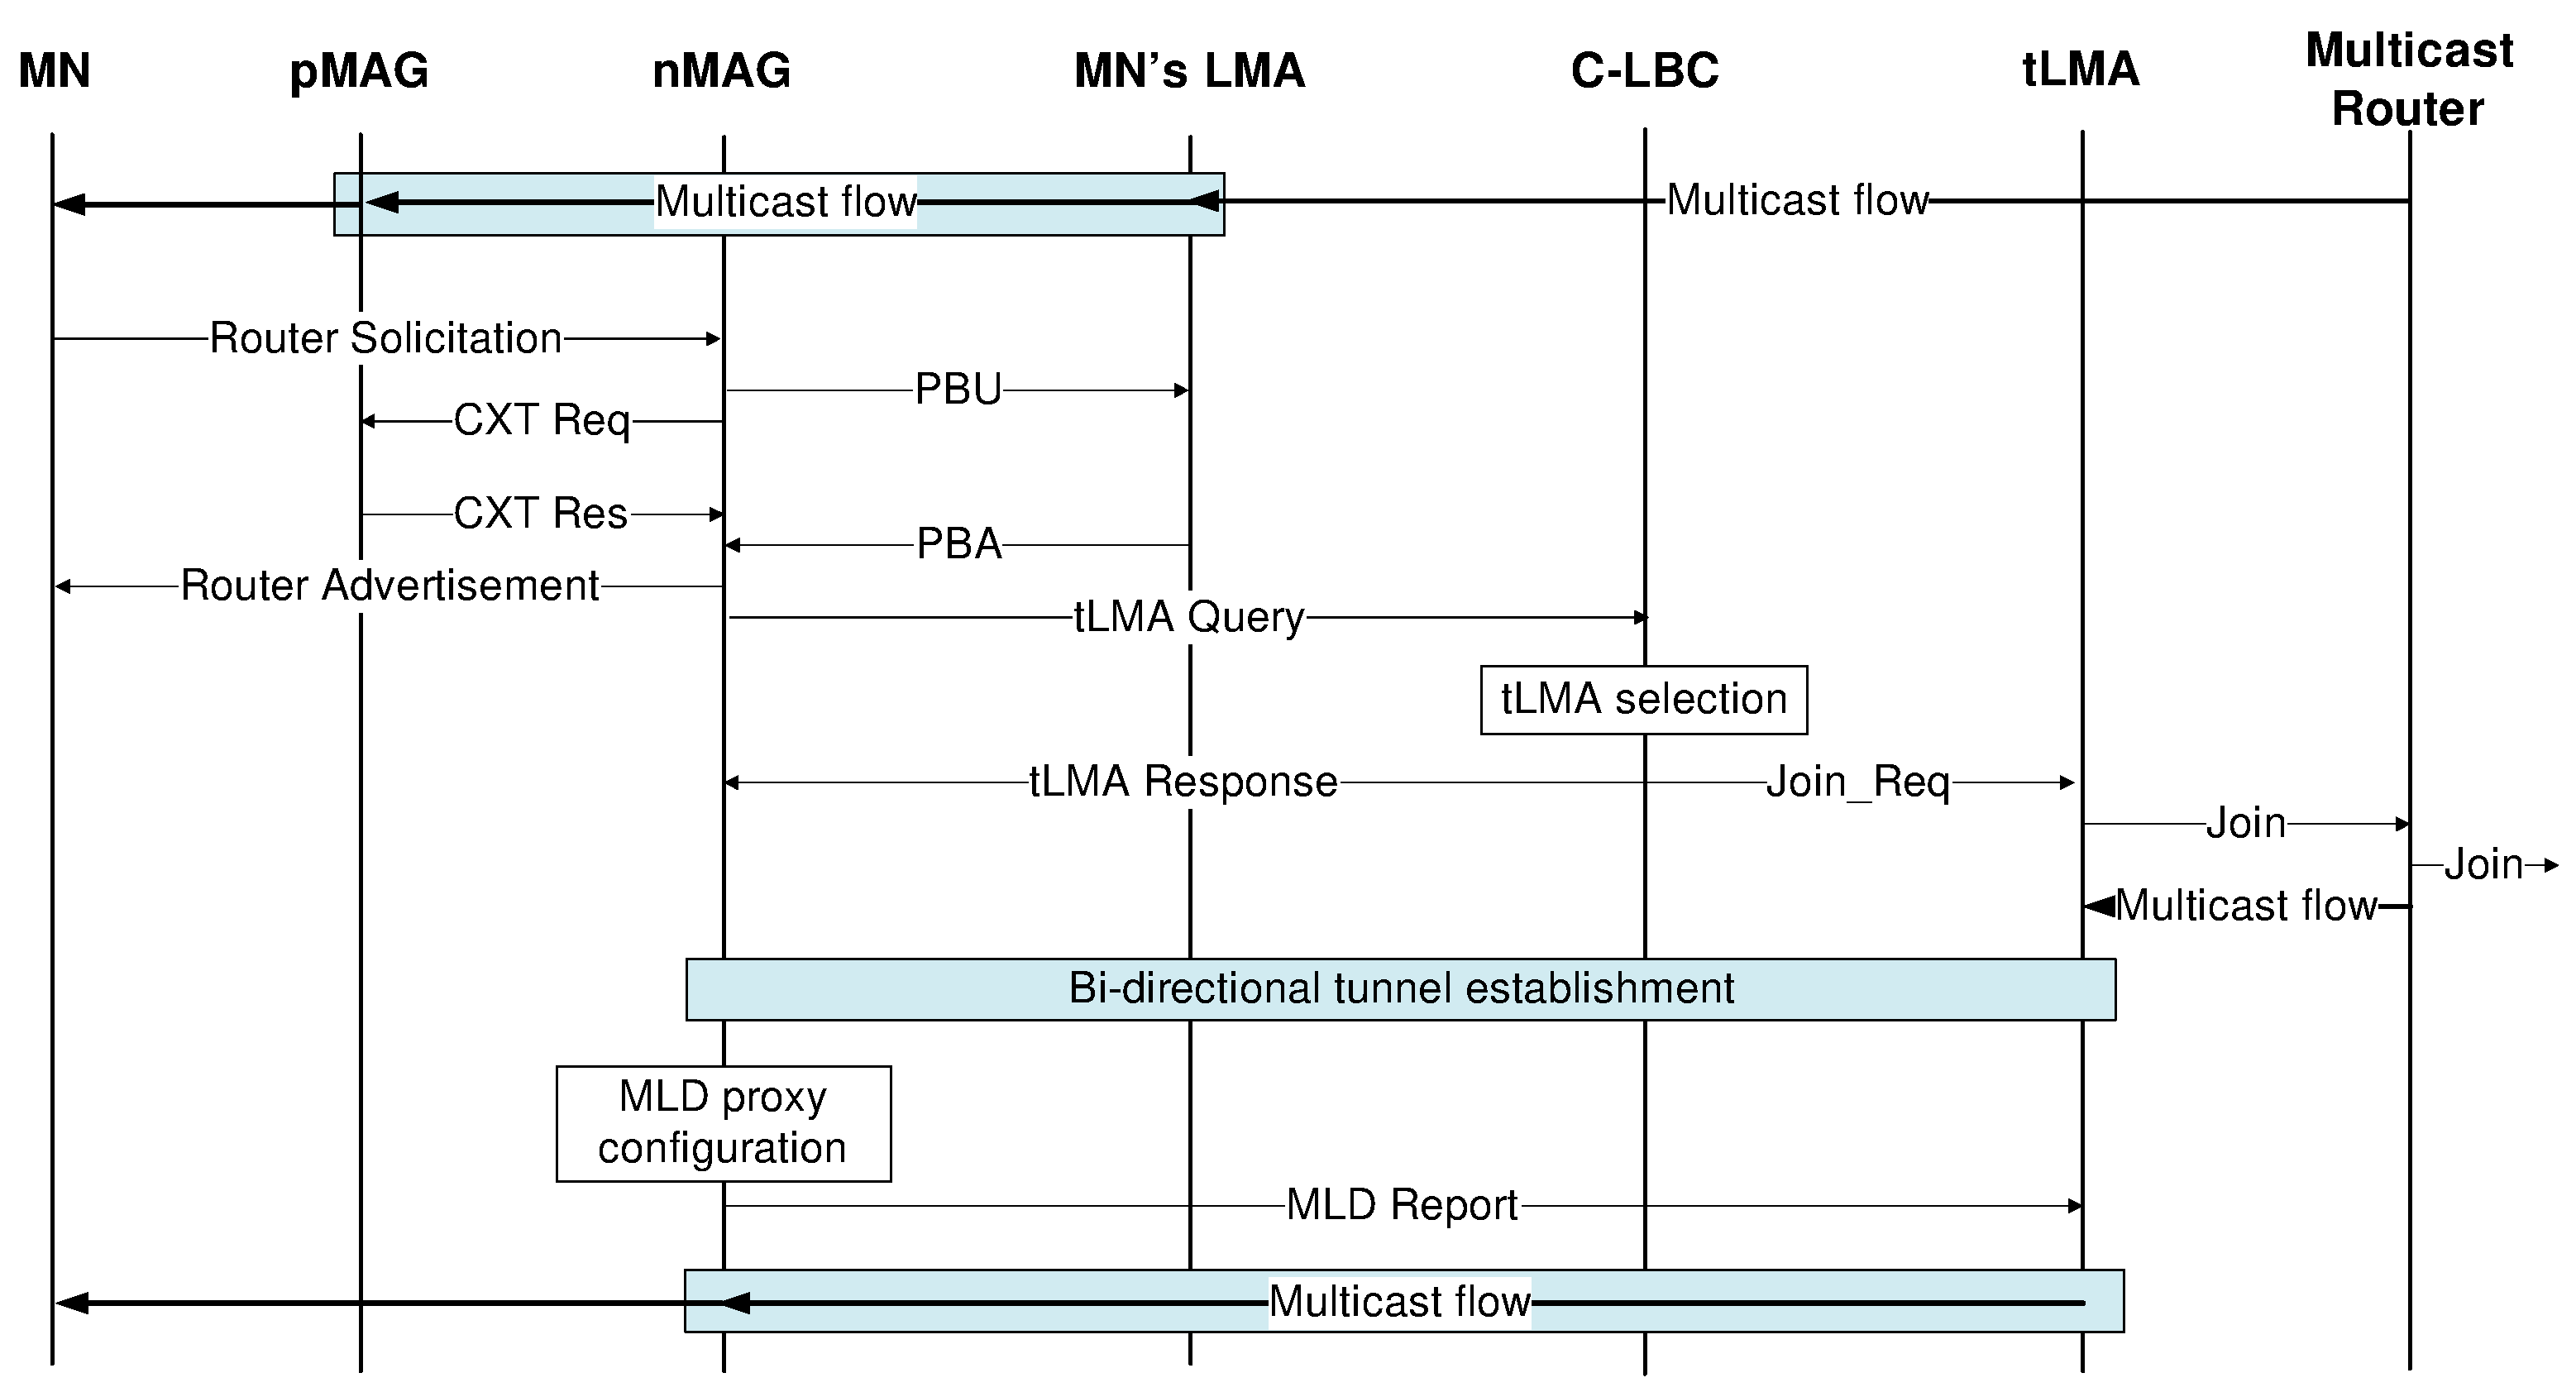
\includegraphics[width=0.70\textwidth]{./Part2/Chapter5/figures/c7_handover_multicast.eps} 
    \caption[Load balancing-related signaling when a node performs a handover in a PMIPv6 domain.]{Handover signaling with LB.}
        \label{fig:handover_multicast}
  \end{center} 
\end{figure}
As can be seen in Fig.~\ref{fig:handover_multicast}, if the MN performs a handover between two MAGs, the normal PMIP operation will be executed to update the routing information at the MN's LMA and the new MAG. Then, the similar process as for the new multicast session at the new MAG will be undertaken to select the appropriate LMAs to serve the ongoing multicast channels.

\section{Performance Analysis}\label{ch7:performance_analysis}
In this section, at first, we will highlight the different load factors imposed on the LMA. Based on that the comparison will be conducted between the reactive-MN and the reactive-multicast approach regarding their efficiency. The multicast service disruption time will also be considered. 
\subsection{Load Analysis}
As stated previously, to support multicast in a PMIPv6 domain, the multicast router (MR) function and the MLD proxy function \cite{RFC_6224} need to be deployed at the LMA and the MAG, respectively. All multicast traffic passes through the MAG-LMA tunnel, accordingly. As such, the load of the LMA comes from two main parts: the load from the typical LMA's tasks ($L_{lma}^{lma}$) and the load from the MR's tasks ($L^{mr}_{lma}$). It is noted that a minor amount of load which is imposed by the background processes (e.g., system processes) is ignored in our analysis.   
Thus, we have\\
\begin{equation}
L_{lma}^{(.)} = L_{lma}^{lma} + L_{lma}^{mr}.
\end{equation}

As a typical LMA, it performs three main logic functions: mobility routing (processing the unicast traffic from/to the associated MNs), location management (processing PBU/PBA, updating binding cache, maintaining tunnel, etc.) and home network prefix (HNP) allocation \cite{PMIPv6}.
As a result, the $L_{lma}^{lma}$ comes from three main parts $L_{lma}^{mor}$, $L_{lma}^{lm}$, and $L_{lma}^{hal}$ corresponding to these logic functions. The $L_{lma}^{mor}$ and $L_{lma}^{hal}$ depend on all the unicast sessions of the registered MNs, and the new MN arrival rate ($\lambda_{n}$), respectively.  While $L_{lma}^{lm}$ depends on the number of registered MNs ($n$) and the new MN arrival rate ($\lambda_{n}$). Hence, they are given by
\begin{eqnarray}
    L_{lma}^{mor}&{} ={}& \sum_{i=1}^{n} \sum_{j=1}^{u_{i}} L_{mn_{i}}^{j},\\
    L_{lma}^{hal}&{} ={}& \lambda_{n} L_{hal},\\
     L_{lma}^{lm}&{} ={}& (n+ \lambda_{n}) L_{lm},
\end{eqnarray}

where $L_{mn_{i}}^{j}$ is the load offered by the unicast flow j of the MN$_{i}$; $L_{lm}$ and $L_{hal}$ are the unit load generated when the LMA performs the location management and HNP allocation for an MN. 

Regarding the multicast router role, the $L_{lma}^{mr}$ can be split into three main contributions corresponding to three functions: packet replication ($L_{mr}^{pr}$), reverse path forwarding (RPF) recalculation ($L_{mr}^{rpf}$,) and state maintenance function ($L_{mr}^{sm}$) \cite{developing_ip_multicast}. The $L_{mr}^{pr}$ is the total load from all the multicast channels which are available at the LMA, and defined as 
 
\begin{equation}
L_{mr}^{pr} = \sum_{i=1}^{m} L_{mc_{i}},
\end{equation}
where $L_{mc_{i}}$ is the load of channel $MC_{i}$.
Note that the multicast router can replicate the data for multiple outgoing interfaces with almost the same level of load compared to that for one interface (or the unicast traffic with the same characteristics e.g., packet size and data rate) \cite{developing_ip_multicast}.  

Let us now consider the different load factors which can be used as the parameters to select the appropriate LMA such as: processor capacity (CPU), number of supported sessions, number of registered MNs, and bandwidth. Accordingly, we assign each factor with a weighting variable which reflects the selected load factors. We then obtain\\
\begin{equation}
L_{lma}^{(.)} = \alpha \left( n + \lambda_{n} \right) L_{lm} + \beta  \lambda_{n} L_{hal} + \gamma \sum_{i=1}^{n} \sum_{j=1}^{u_{i}} L_{mn_{i}}^{j}  + \delta L_{mr}^{rpf} + \theta  L_{mr}^{sm} + \rho  \sum_{i=1}^{m} L_{mc_{i}}. 
\label{lma_load}
\end{equation}

where $\alpha, \beta, \gamma, \delta, \theta$, and $\rho$ are weighting factors (in the interval [0,1]). For example, if the load is defined as the number of registered MNs, only two factors $L_{lma}^{lm}$ and $L_{lma}^{hal}$ are taken into account. In this case, the values of $\gamma, \delta, \theta, \rho$ should be set to 0. LMA load is given as\\
\begin{equation}
L_{lma}^{(.)} = \alpha \left( n+ \lambda_{n} \right) L_{lm} + \beta \lambda_{n} L_{hal}. 
\label{eg:load_mn}
\end{equation}

As a result, the impact of the number of sessions as well as the session's data rates on the LMA load are ignored. Similarly, if the load is considered as the number of sessions, the $L_{lma}^{mor}$ and $L_{mr}^{pr}$ are taken into consideration, in which the load of each session is identical. Thus, $\alpha, \beta, \delta$, and $\theta$ should be set to 0. Eg.~(\ref{lma_load}) becomes  \\
\begin{equation}
L_{lma}^{(.)} = \gamma \sum_{i=1}^{n} \sum_{j=1}^{u_{i}} L_{mn_{i}}^{j} + \rho \sum_{i=1}^{m} L_{mc_{i}}. 
\end{equation}

Again, the impact of the session's data rate is ignored. However, it is obvious that a high data rate session puts much more load on the LMA than the low data rate one. Therefore, they cannot be treated equally. In this chapter, we consider the sessions with different characteristics have different impact on the load. 

In order to evaluate the load distribution among LMAs in different approaches, we use Jain's Fairness Index \cite{jain-index}. Let L denote the set of LMAs in the domain: $L=\lbrace LMA_{1},..,LMA_{l}\rbrace$, where l is the number of LMAs. According to \cite{jain-index}, the fairness index can be computed by\\
\begin{equation}
FI = \dfrac{(\sum_{i=1}^{l} L_{lma}^{(i)})^{2}}{l \cdot \sum_{i=1}^{l} (L_{lma}^{(i)})^{2}},
\end{equation} 
where $L_{lma}^{(i)}$ is the load of the $LMA_{i}$ (i=1,..,l).
The fairness index ranges from $\frac{1}{l}$ to 1, in which the higher index indicates more fair situation. Ideally, when the load is equally distributed among LMAs, the fairness index is 1.
    
\subsection{Multicast Service Disruption Consideration}
\begin{figure}[tb!] 
  \begin{center} 
    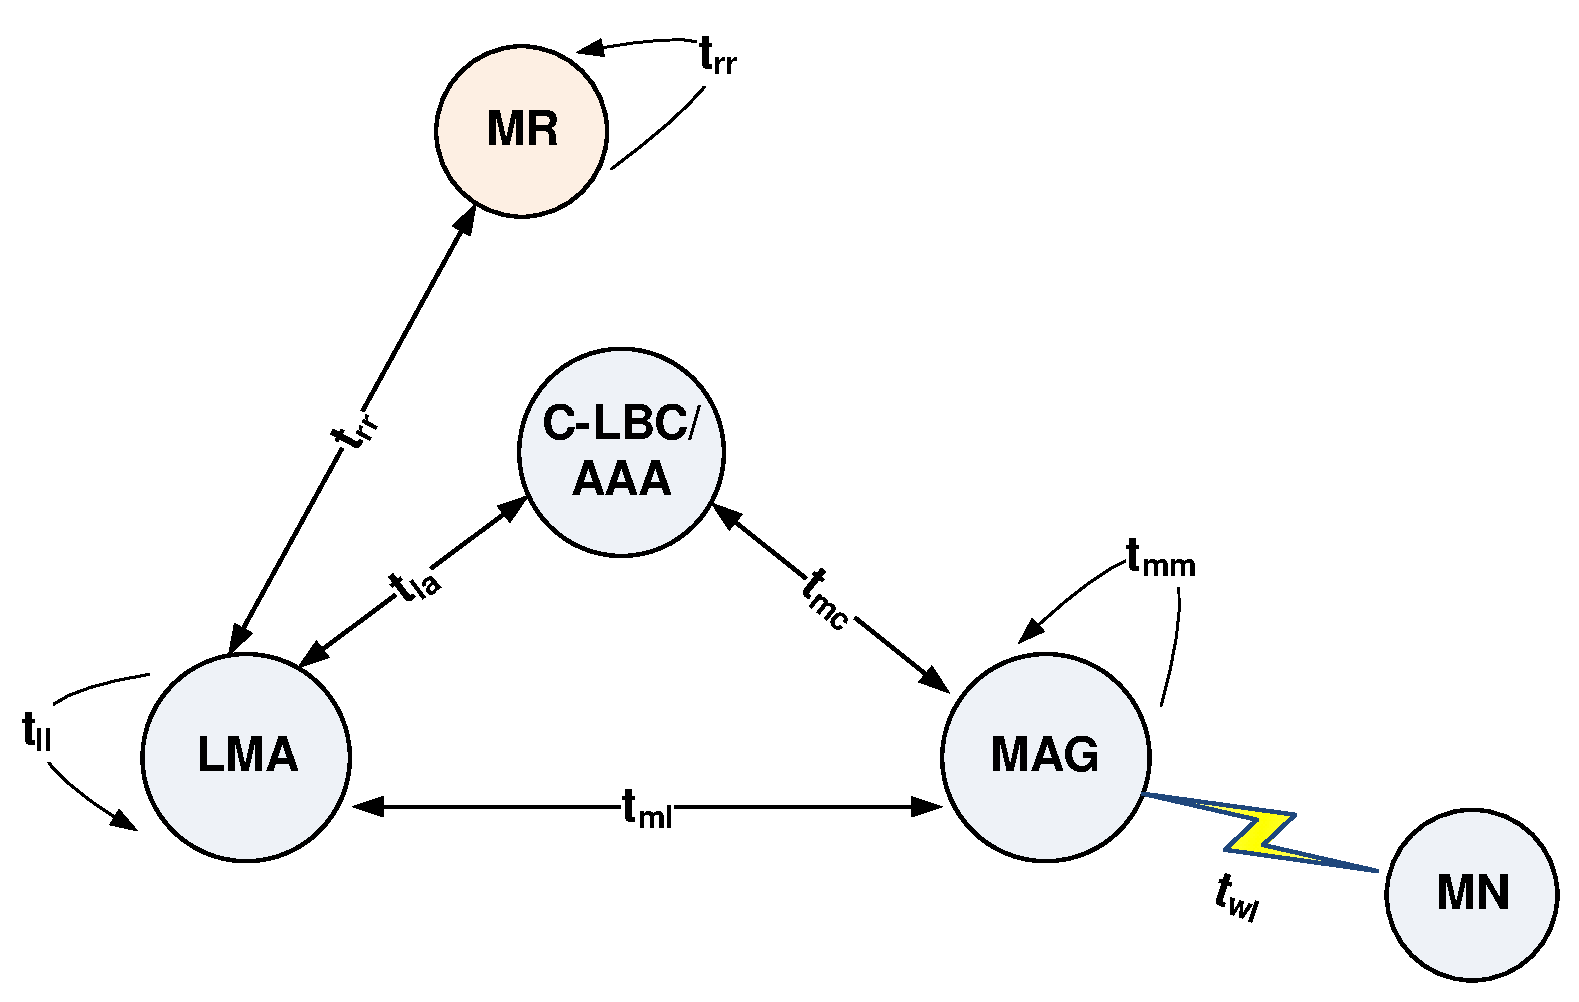
\includegraphics[width=0.52\textwidth]{./Part2/Chapter5/figures/topology_analysis.eps} 
    \caption[Reference network topology for multicast service disruption analysis: from the load balancing perspective]{Reference network topology.}
    \label{fig:topology_analysis}
  \end{center} 
\end{figure}
In the reactive-MN and the reactive-multicast approach, the changing LMA of an MN (listener) may cause the service disruption of the ongoing multicast sessions. The multicast service disruption time is defined as a period when a listener cannot receive the multicast packets. Fig.~\ref{fig:topology_analysis} shows a reference topology for performance analysis. The delay factors consisting of the total
delay are defined as follows:
\setlength \abovedisplayskip{-1pt}
\vspace{-0.1in}
\begin{itemize}
\itemsep 0.07em
\item $t_{mm}$: the delay between two MAGs.
\item $t_{ml}$: the delay between MAG and LMA.
\item $t_{mc}$: the delay between MAG and C-LBC.
\item $t_{la}$: the delay between LMA and AAA/C-LBC.
\item $t_{ll}$: the delay between two LMAs. 
\item $t_{rr}$: the delay between two MRs (between LMA and MR).
\item $t_{wl}$: the delay between MAG and listener (MN) (wireless connection).
\item $t_{join}$: the delay time an MR needs to join a multicast channel (including processing time and PIM Join transmission time).
\item $t_{qrd}$: the query response delay which is the interval between the moment when the MN receives an MLD Query and replies with an MLD Report \cite{MLDv2}.
\item $t_{cv}$: the routing convergence time which reflects the time to update the new anchor location of the selected MN's prefix.
\end{itemize}

In the reactive-MN approach, as can be seen in Fig.~\ref{fig:reactive_MN_flow}, the service disruption time ($SD$) can be calculated from the moment when the cLMA sends a PBU to the tLMA until the moment when the MN receives the first multicast packet from the tLMA. Let $d_{join}$ and $d_{delivery}$ denote the time needed for the tLMA to join and get the first multicast packet for this channel (from a router which already had the multicast forwarding state for this group, namely intersection MR or IMR), respectively. Assuming that $n_{mr}$ is the average number of hops between tLMA and IMR, we have 
\begin{equation}
d_{join} = n_{mr} t_{join},
\end{equation}
\begin{equation}
d_{delivery} = n_{mr} t_{rr}.
\end{equation}

Thus, the service disruption time in the reactive-MN approach is given by\\
\begin{equation}
SD_{R\_MN} = 2t_{ll} + 3t_{ml} + 3t_{wl} + t_{qrd} + n_{mr} t_{join} + n_{mr} t_{rr} + t_{cv}. 
\label{eq:r_mn}
\end{equation}

Via the utilization of the peering function (PF) in the reactive-MN approach, the time needed for the MLD proxy instance at the MAG to obtain the multicast subscription information can be ignored. Consequently, the service disruption can be calculated as\\
\begin{equation}
SD_{R\_MN\_PF} = 2t_{ll} + 3t_{ml} + t_{wl}  + n_{mr} t_{join} + n_{mr} t_{rr} + t_{cv}.
\label{eq:r_mn_pf}
\end{equation}

Similarly, the service disruption time in the reactive-multicast approach is computed from the moment when the cLMA sends a load warning message to the MAG until the moment when the MN receives the multicast traffic (see Fig.~\ref{fig:reactive_multicast}).\\
\begin{equation}
SD_{R\_M} = max \{2t_{ml}, n_{mr} t_{join} + n_{mr} t_{rr}\} + t_{ml} + t_{wl}.
\label{eq:r_m}
\end{equation}

Also, as seen in Fig.~\ref{fig:handover_multicast}, the service disruption during handover (multicast handover latency) when applying the multicast-based LB mechanism is expressed as\\
\begin{multline}
SD_{HO} = D_{L2} + 2t_{wl} + max \{2t_{ml}, 2t_{mm}\} + t_{mc} \\+max \{t_{mc} +t_{ml}, t_{la} + n_{mr} t_{join} + n_{mr} t_{rr}\} + t_{ml}.
\label{eq:ho}
\end{multline}

\section{Experimentation}\label{c7:experiment}
From the LB perspective, this section will present two separate experiments. At first, we will show in general how the different factors affect the load of an LMA. We will then evaluate the performance of the multicast-based solution in comparison with the MN-based solution and the pure-PMIP environment (without any load balancing mechanism) by using a near-to-real testbed. It is noted that, at this stage, we only focus on the case where the traffic is dominated by the multicast traffic. In addition, the load is defined as the CPU utilization rate and the performance metric is the load distribution among the LMAs. From the multicast perspective, this section will present the numerical results for the service disruption time analysis given in the previous section. 

\subsection{Experimentation Setup and Scenarios Description}
\begin{figure}
\centering
\subfloat[]{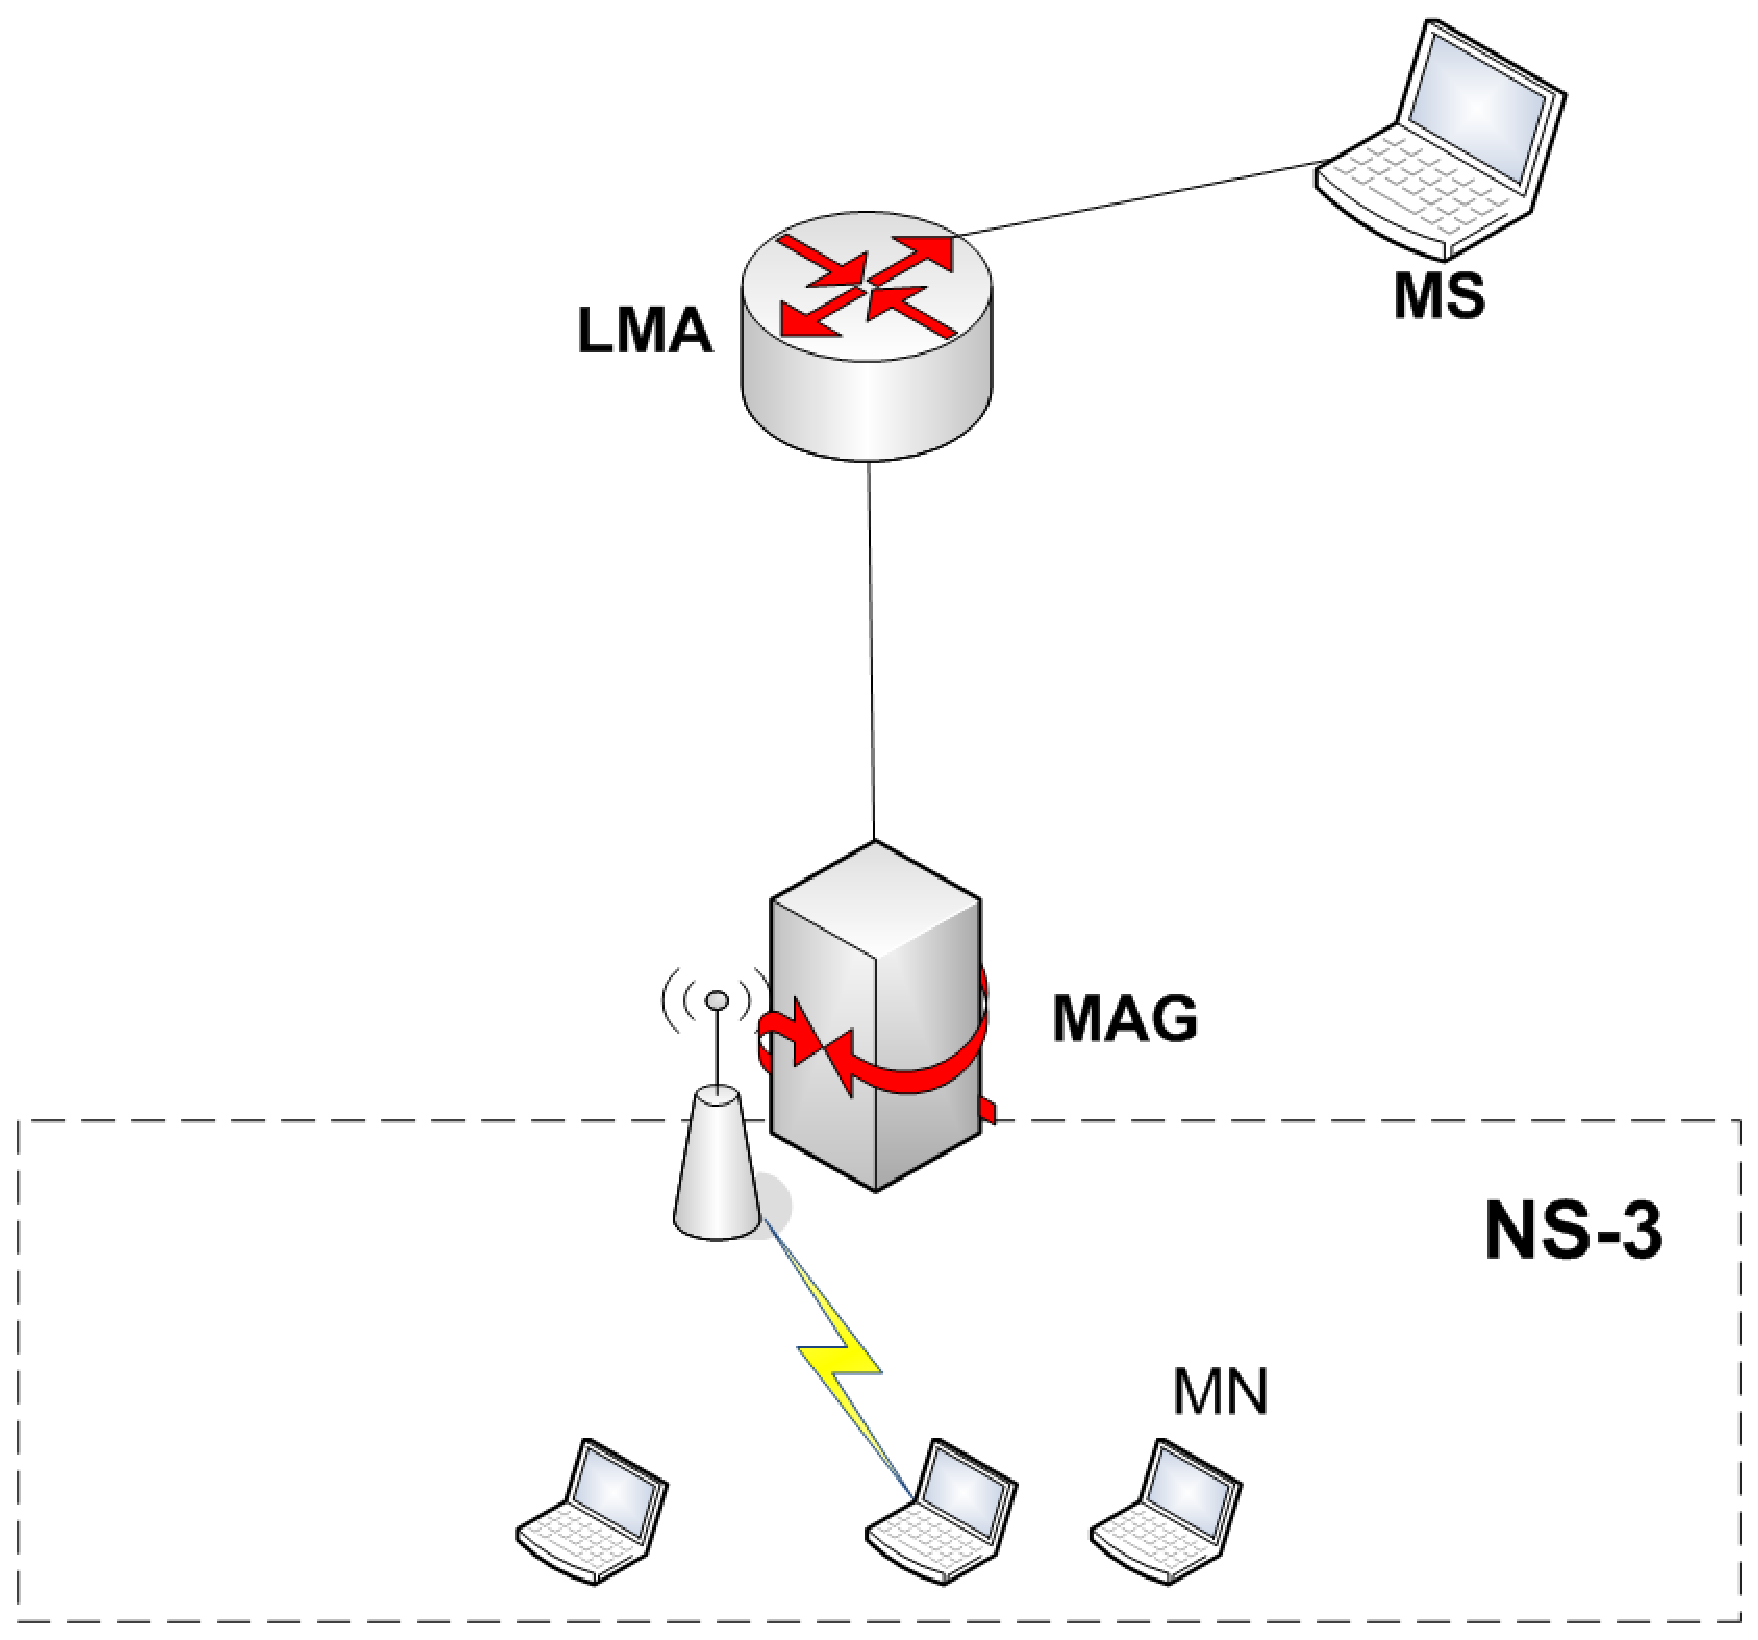
\includegraphics[width=0.35\textwidth]{./Part2/Chapter5/figures/testbed-measurement.eps} \label{fig:testbed-measurement}}\,
\subfloat[]{\includegraphics[width=0.47\textwidth]{./Part2/Chapter5/figures/testbed.eps}\label{fig:testbed-multicast}}
\caption[Testbeds for load balancing mechanisms. ]{Testbeds: (a) Experiment 1, (b) Experiment 2}
\label{fig:testbed}
\end{figure}

As illustrated in Fig.~\ref{fig:testbed}, the testbed is deployed as similar as in Chapter \ref{ch:multicast_PMIP}. The PMIP entities (LMA, MAG) and the multicast sources (MSs) are the virtual machines while the access points (APs) and MNs, which play the role of a multicast listener, are NS-3 nodes. During the experimentation, the LMA load is collected by using a performance measurement tool e.g., \textit{mpstat}\footnote{http://linuxcommand.org/man\_pages/mpstat1.html}. To improve the credibility of the experiment results, the LMA load was collected every one second during 360 seconds in each experiment. 

To generate the multicast traffic, several tools can be used e.g., \textit{Iperf} \cite{iperf} and \textit{MINT} \cite{mint} (and \textit{mcfirst}\footnote{mcfirst command: http://manpages.ubuntu.com/manpages/precise/man1/mcfirst.1.html}). 
For example, in case of \textit{Iperf},  the following Linux commands can be used: \\
\textit{Source\# Iperf -s -u -B ff08::1 -V -i 1}\\
\textit{Listener\# Iperf -c ff08::1 -V -u -T 32 -t 100 -i 1 -l 67B -p 12345}

In case of using \textit{MINT} and \textit{mcfirst}: \\
\textit{Source\# ./mint -s -p 1234 -n 1000 -6 -t 12 ff08::2}\\
\textit{Listener\# mcfirst -6 -I eth0 ff08::1 1234}
\subsubsection{Impact of Different Load Factors} 
To show the impact of different factors on the LMA load, the first experiment used a testbed composing of one LMA, one MAG (and one AP), and one MS, as described in Fig.~\ref{fig:testbed-measurement}. Then two experiment scenarios are defined. The scenario 1 aims at demonstrating the case when the load takes into account only the number of MNs. The number of MNs associated with the LMA will be varied from 1 to 150 (Due to the limitation of the testbed, it can only support upto 150 MNs). The binding registration signaling for these MNs occurred within a small interval (50s) which almost represents the worst case scenario.  The scenario 2 shows the impact of unicast/multicast flow with different data rates on the LMA load. Thus, only one MN is required. At first, the MN subscribes to a multicast channel broadcasting by the MS. The LMA load will be measured when the flow's data rate is varied from 100 Kbps to 15 Mbps. Note that a standard definition video streaming typically runs at 3.75 Mbps while the high definition at 15 Mbps \cite{multicast-bandwidth}. The multicast flow is then replaced by the unicast one with the same data rate. The datagram size in both cases is kept constant at 67 bytes.
\subsubsection{Evaluation of the Multicast-based LB Mechanism}
The second experiment aims at evaluating the performance of the multicast-based solution in comparison with the MN-based and the pure-PMIP environment. At this stage, the experiment focuses on the case where the traffic is dominated by the multicast traffic. The performance evaluation metric is the load distribution among LMAs. This metric is selected since we could not achieve high system performance without fairly and efficiently utilizing the available network resources. The other metrics such as queuing delay and packet dropping probability will be left for future works. 

As illustrated in Fig.~\ref{fig:testbed-multicast}, the testbed is composed of one LBC, three LMAs, three MAGs (and three APs), three MSs, and 18 MNs. The C-LBC functionality is implemented by extending the LMA functionality. At the beginning, each multicast source $MS_{i}$ (i=1,2,3) broadcasts six multicast channels $C_{ij}$ (j=1,..,6) with identical traffic characteristics (400 Kbps). In the experiment, we use the same threshold value for all LMAs, for example, 85 percent of the CPU utilization rate. At first, the $MN_{ij}$ attaches to the $MAG_{i}$ and the $LMA_{i}$, respectively. The unicast flow is also created between each MN and the corresponding MS (100 Kbps). Two scenarios are then defined to evaluate the proactive-multicast and the reactive-multicast approach. 

In the scenario 1, six $MN_{1j}$ (j=1,..,6) join six multicast channels $C_{1j}$ (via $LMA_{1}$); $MN_{21}$ joins $C_{21}$ (via $LMA_{2}$); $MN_{31}$ and $MN_{32}$ join $C_{31}$, $C_{32}$ (via $LMA_{3}$), respectively. Three approaches are considered: the pure-PMIP, the proactive-MN and the proactive-multicast.
In the scenario 2, six $MN_{ij}$ (j=1,..,6) join three multicast channels (say $C_{i1}$, $C_{i2}$, $C_{i3}$) at the $LMA_{i}$ (i=1,2,3) (two MNs per channel, three channels at each LMA). Then the data rate of the existing multicast sessions as well as the number of sessions are varied to make the LMA load changes. For instance, at the $LMA_{1}$ the data rate of the channel $C_{11}$ and $C_{12}$ is increased with 800 Kbps and 1.2 Mbps, respectively. The channel $C_{21}$ (at $LMA_{2}$) and the channels $C_{31}$, $C_{32}$ (at $LMA_{3}$) are terminated. The results then are collected when the pure-PMIP, the reactive-multicast and the reactive-MN approach are applied.

\subsection{Experimental Results}
\subsubsection{Load Factors Measurement}
\begin{figure}[h!]
\centering
\subfloat[]{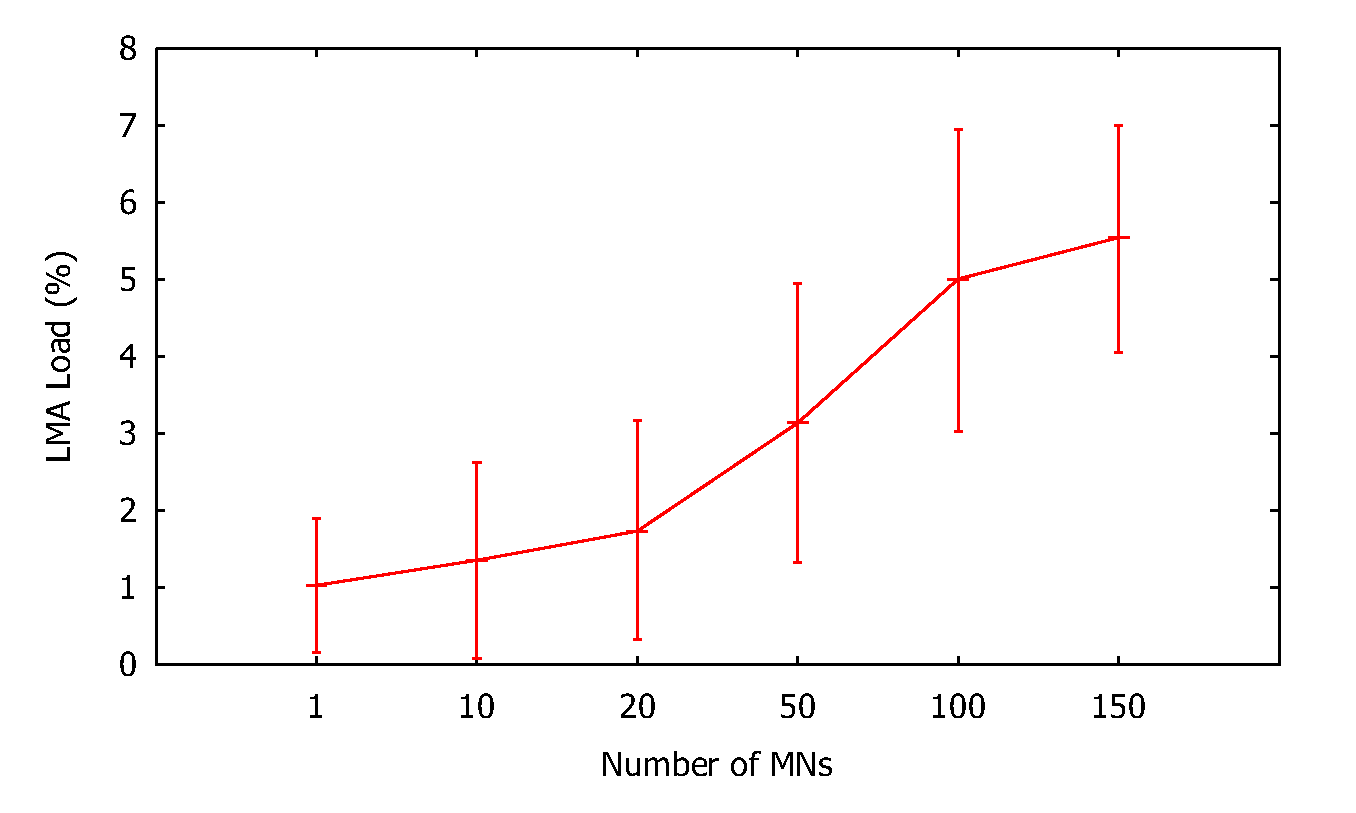
\includegraphics[width=0.47\textwidth]{./Part2/Chapter5/figures/lma_mn.eps} \label{fig:lma_mn}}\,\,\,\,\,\,
\subfloat[]{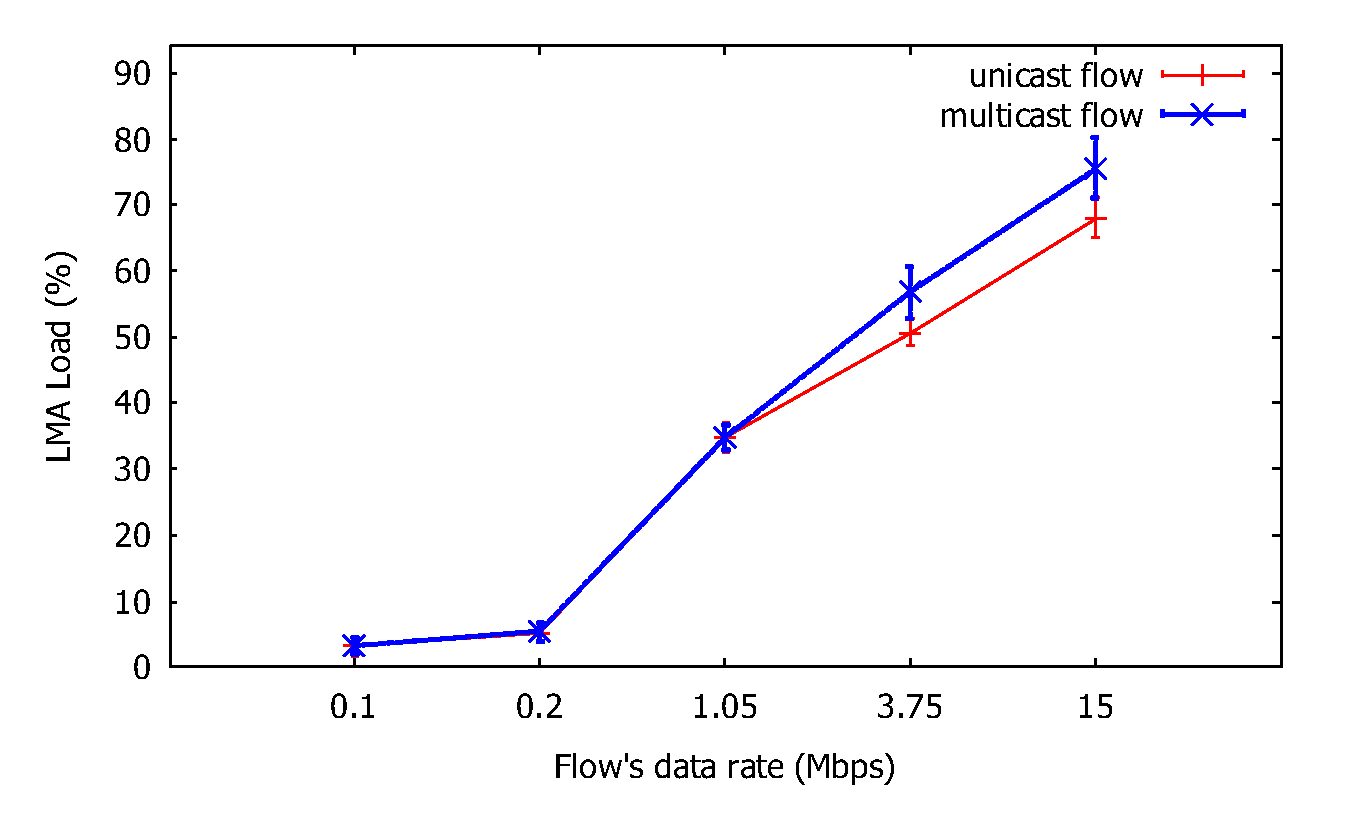
\includegraphics[width=0.47\textwidth]{./Part2/Chapter5/figures/unicast_multicast.eps}\label{fig:unicast_multicast}}
\caption[Load factors measurement.]{Experiment 1: (a) load .vs number of MNs, (b) unicast .vs multicast flow.}
\label{fig:experiment1}
\end{figure}
Fig.~\ref{fig:lma_mn} reports the average and standard deviation values of LMA load as a function of the number of MNs (scenario 1). In this case, the load is calculated according to Eq.~(\ref{eg:load_mn}). We also measure the load from background processes: (average, standard deviation) = (1.001\%, 0.888\%). We can observe that the load slightly increases when the number of MNs increases. Fig.~\ref{fig:unicast_multicast} illustrates the LMA load when the data rate of the multicast and unicast flow is varied (scenario 2). When the flow's data rate is low, the load imposed by the multicast and unicast flow is almost the same.  As the flow rate increases, the load offered by the multicast flow is higher than that by the unicast flow. As the experiment was conducted by using a very limited capacity machine, it requires about 75\% load to treat a high definition video flow (15 Mbps). 
It also could be observed that the load offered from a typical LMA's task with 150 MNs is similar to that from a low rate multicast flow (about 200 Kbps). Thus, it is obvious that the multicast/unicast flow is a crucial factor in terms of load put on the LMA. In other words, in a multicast-dominated domain, moving an MN from the overloaded LMA could not help reduce its load significantly. 
\subsubsection{Evaluation of the Multicast-based Load Balancing Solution}
Fig.~\ref{fig:fi_proactive} shows the FI value in the scenario 1. At the beginning, the load of all LMAs is almost the same. As a result, the FI value is very close to 1 (indicating that the load is almost shared among the LMAs). From the time the MNs subscribed to the multicast channels (at about 120s), the FI value is decreased rapidly in the pure-PMIP environment since the load is concentrated on the $LMA_{1}$. For instance, the $LMA_{1}$ becomes overloaded while the $LMA_{2}$ and $LMA_{3}$ are at low load. Since the LMA assignment is already done for the MNs, the FI value in the pure-PMIP can also be considered as that in the proactive-MN. We observed that the FI value in the multicast-based approach is always greater than that in the other cases. Also, the FI value is close to 1. It demonstrates that the multicast-based approach achieves a better load distribution among the LMAs. The reason is the proactive-multicast approach dynamically assigns the channel to the least loaded LMA at the time when the channel is started. 
\begin{figure}[h!]
\centering
\subfloat[]{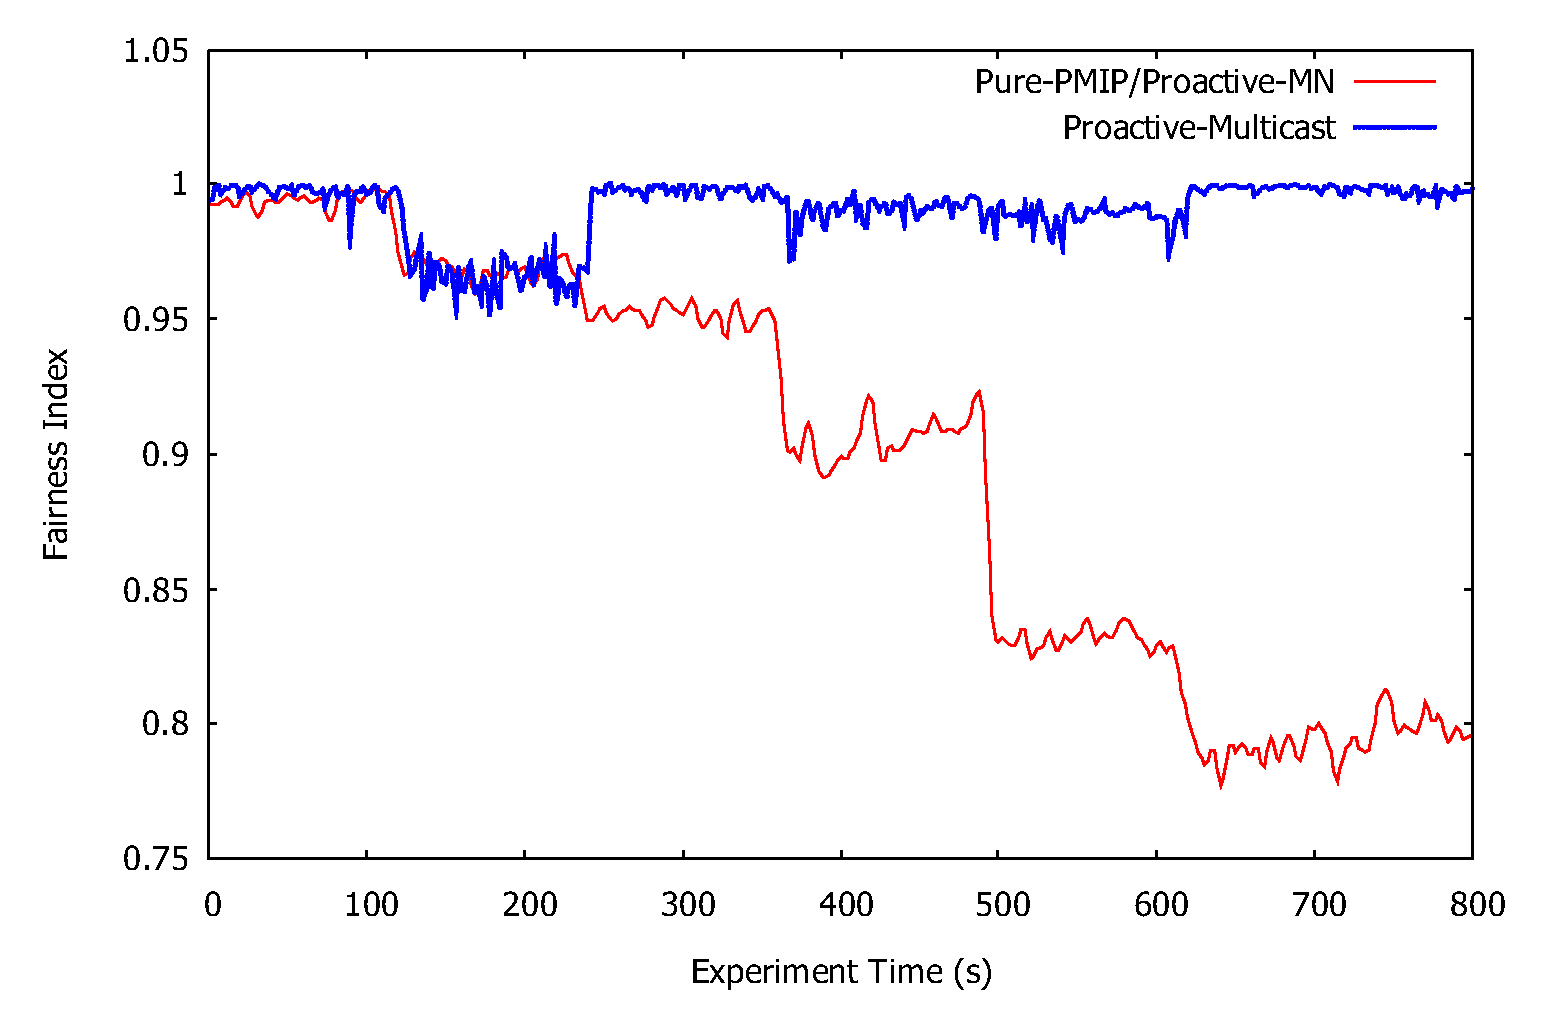
\includegraphics[width=0.47\textwidth]{./Part2/Chapter5/figures/fi_proactive.eps} \label{fig:fi_proactive}}\,
\subfloat[]{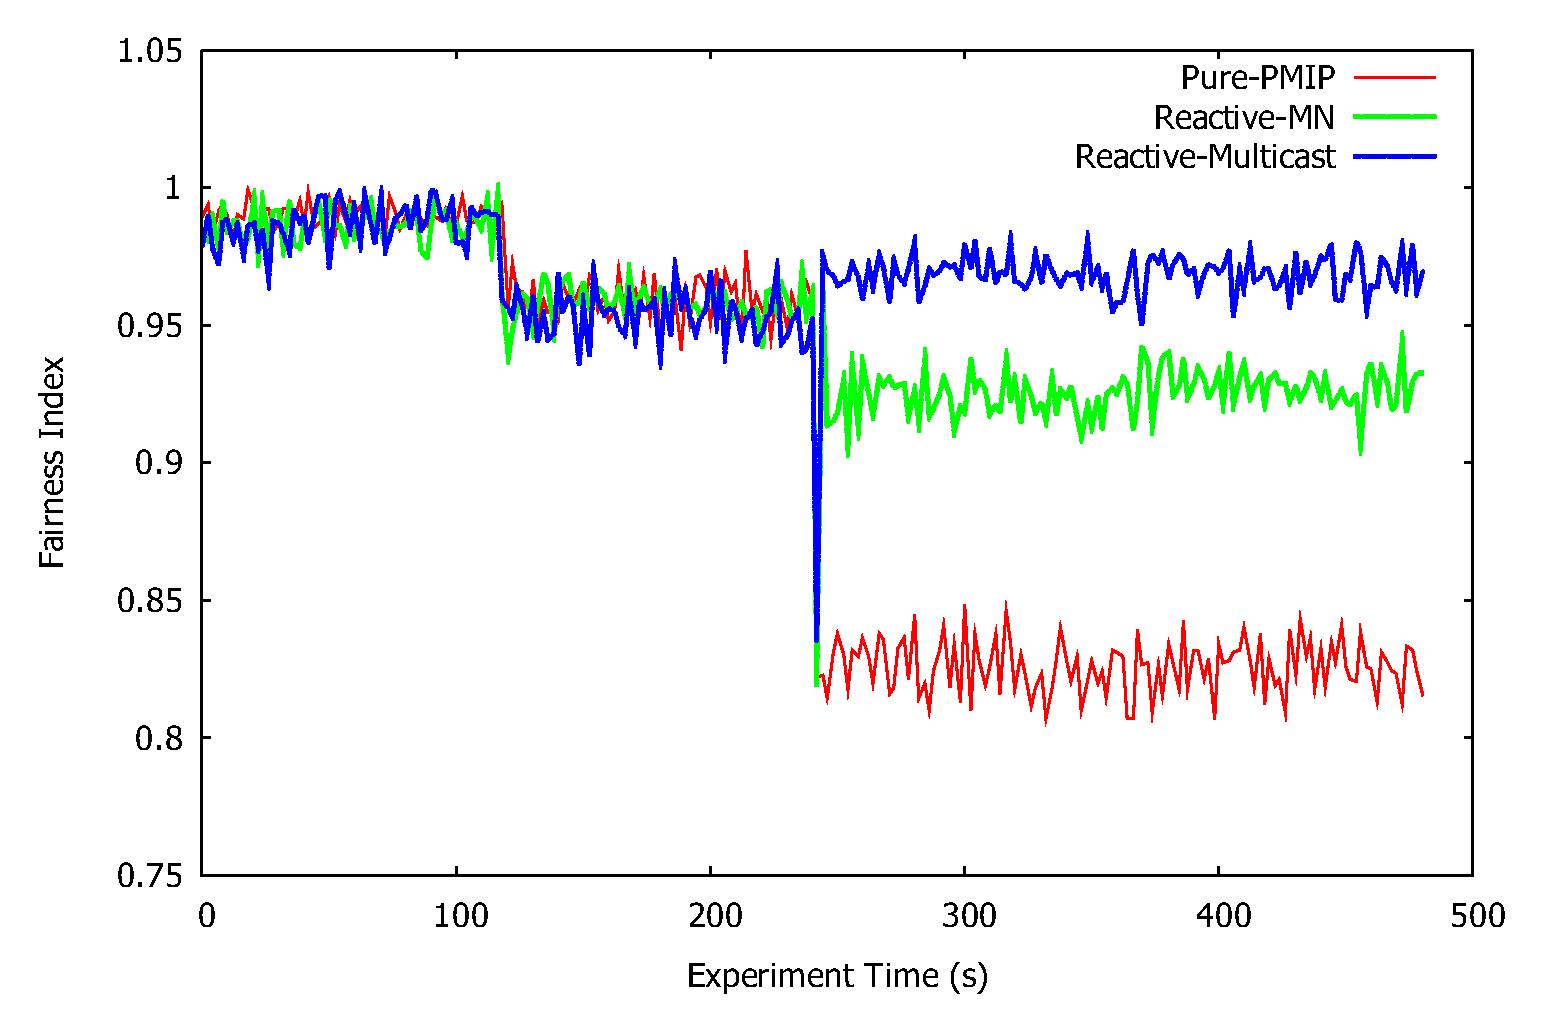
\includegraphics[width=0.47\textwidth]{./Part2/Chapter5/figures/fi_reactive.eps}\label{fig:fi_reactive}}
\caption[Fairness Index for the multicast-based load balancing mechanisms.]{FI value in the experiment 2: (a) Scenario 1, (b) Scenario 2.}
\label{fig:scenario1}
\end{figure}

Fig.~\ref{fig:fi_reactive} plots the FI value in the scenario 2. At the beginning (from 0 to 120 ms), when each LMA has to serve three identical channels, the LMAs' load is nearly equal. As a result, the FI value in three approaches is almost the same and very close to 1. 
As the data rate of the existing multicast flow in $LMA_{1}$ is increased ($C_{11}$'s data rate is increased from 400 Kbps to 800 Kbps), $LMA_{1}$ load is increased accordingly. Meanwhile, the load of $LMA_{2}$ and $LMA_{3}$ is decreased (channel $C_{21}$ at $LMA_{2}$ and $C_{31}$ at $LMA_{3}$ are terminated). Consequently, the FI value is decreased. Since the reactive LB mechanism is only evolved when the LMA load exceeds the threshold value (85\%), the FI values in three approaches are kept the same when the LMAs are running under a heavy load. When $LMA_{1}$ is overloaded (at about 240s, as $C_{22}$'s data rate is increased from 400 Kbps to 1.2 Mbps), the LB mechanism is involved. As a result, the FI value in the reactive-MN and reactive-multicast is clearly greater than that in the pure-PMIP environment. That means the load is better shared between the LMAs. Moreover, the reactive-multicast approach gives a better performance than the MN-based (FI value is greater). In more details, the multicast channel with the highest data rate ($C_{12}$ with 1.2 Mbps) is moved from $LMA_{1}$ to $LMA_{3}$ in the reactive-multicast approach, while one MN (among two) subscribed to this channel is moved to $LMA_{3}$ in the reactive-MN approach. 
\begin{figure}[h!]
\centering
\subfloat[]{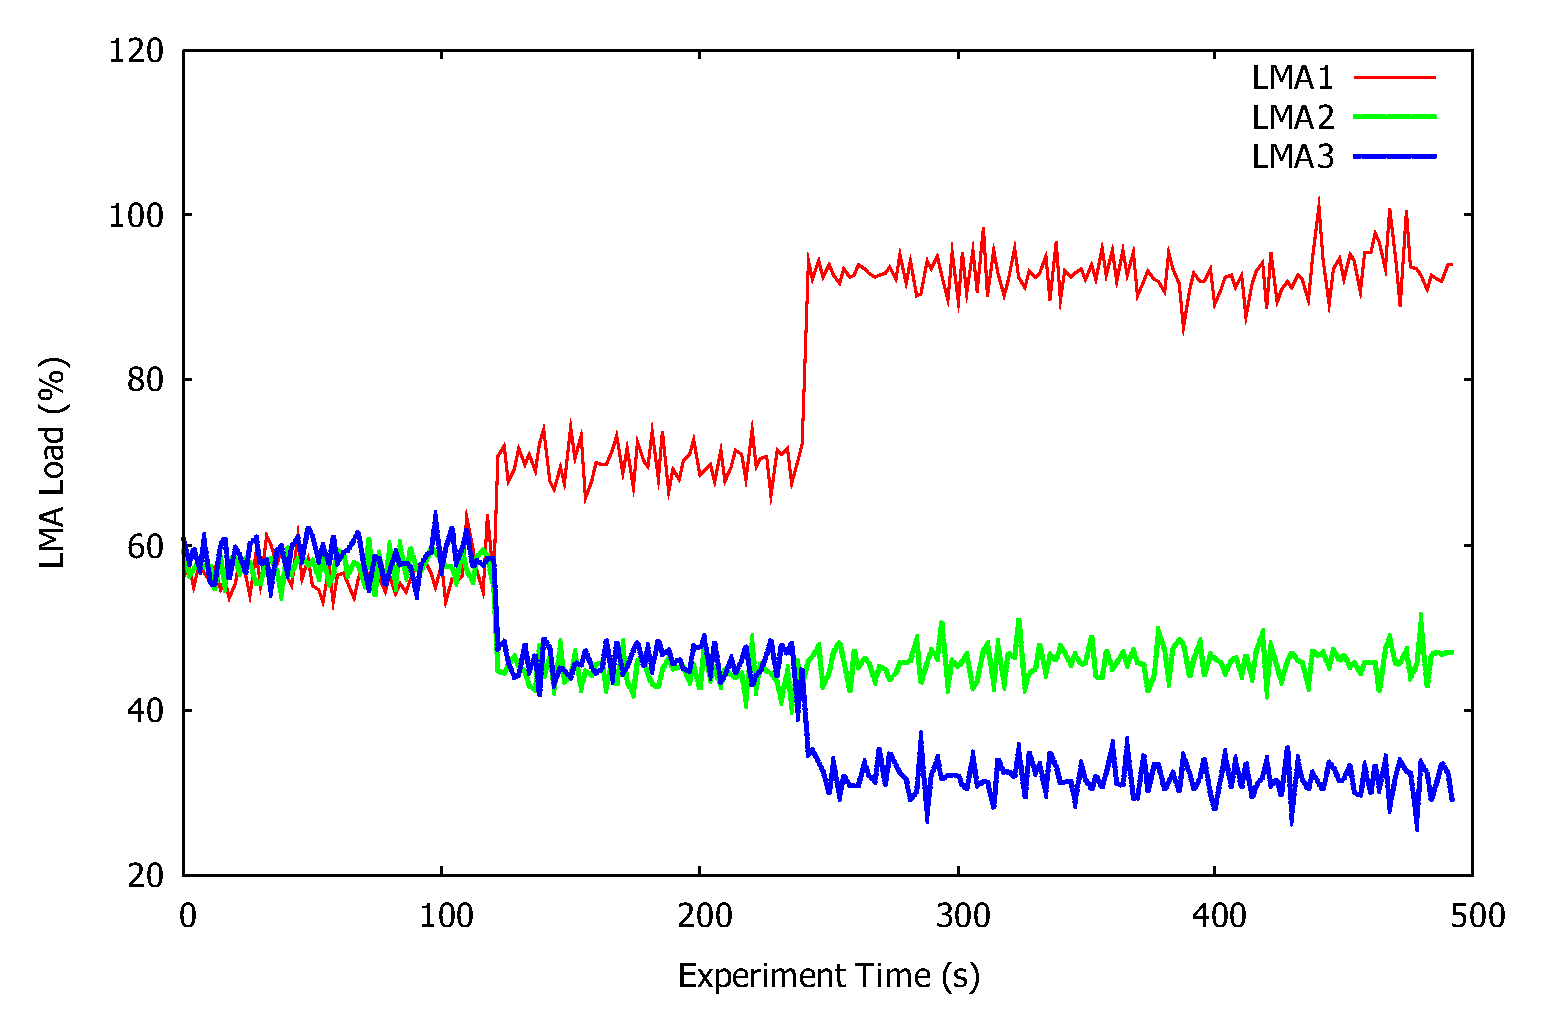
\includegraphics[width=0.35\textwidth]{./Part2/Chapter5/figures/reactive_PMIP_result.eps} \label{fig:s2_pure_pmip}}
\subfloat[]{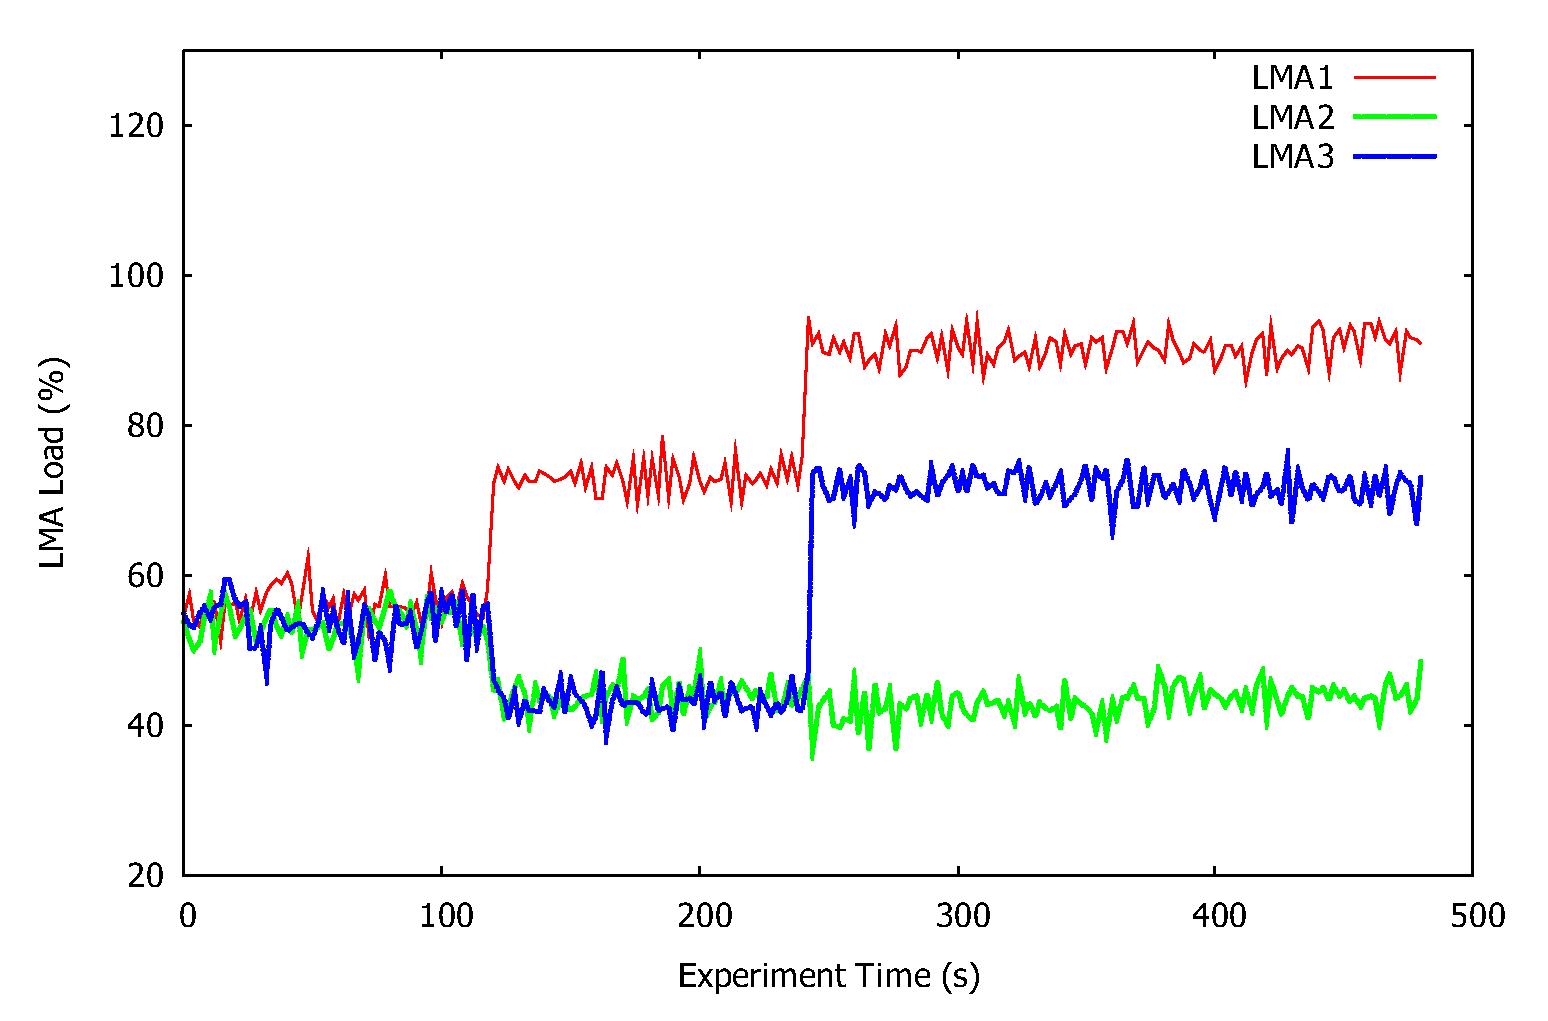
\includegraphics[width=0.35\textwidth]{./Part2/Chapter5/figures/reactive_mn.eps}\label{fig:s2_reactive_mn}}
\subfloat[]{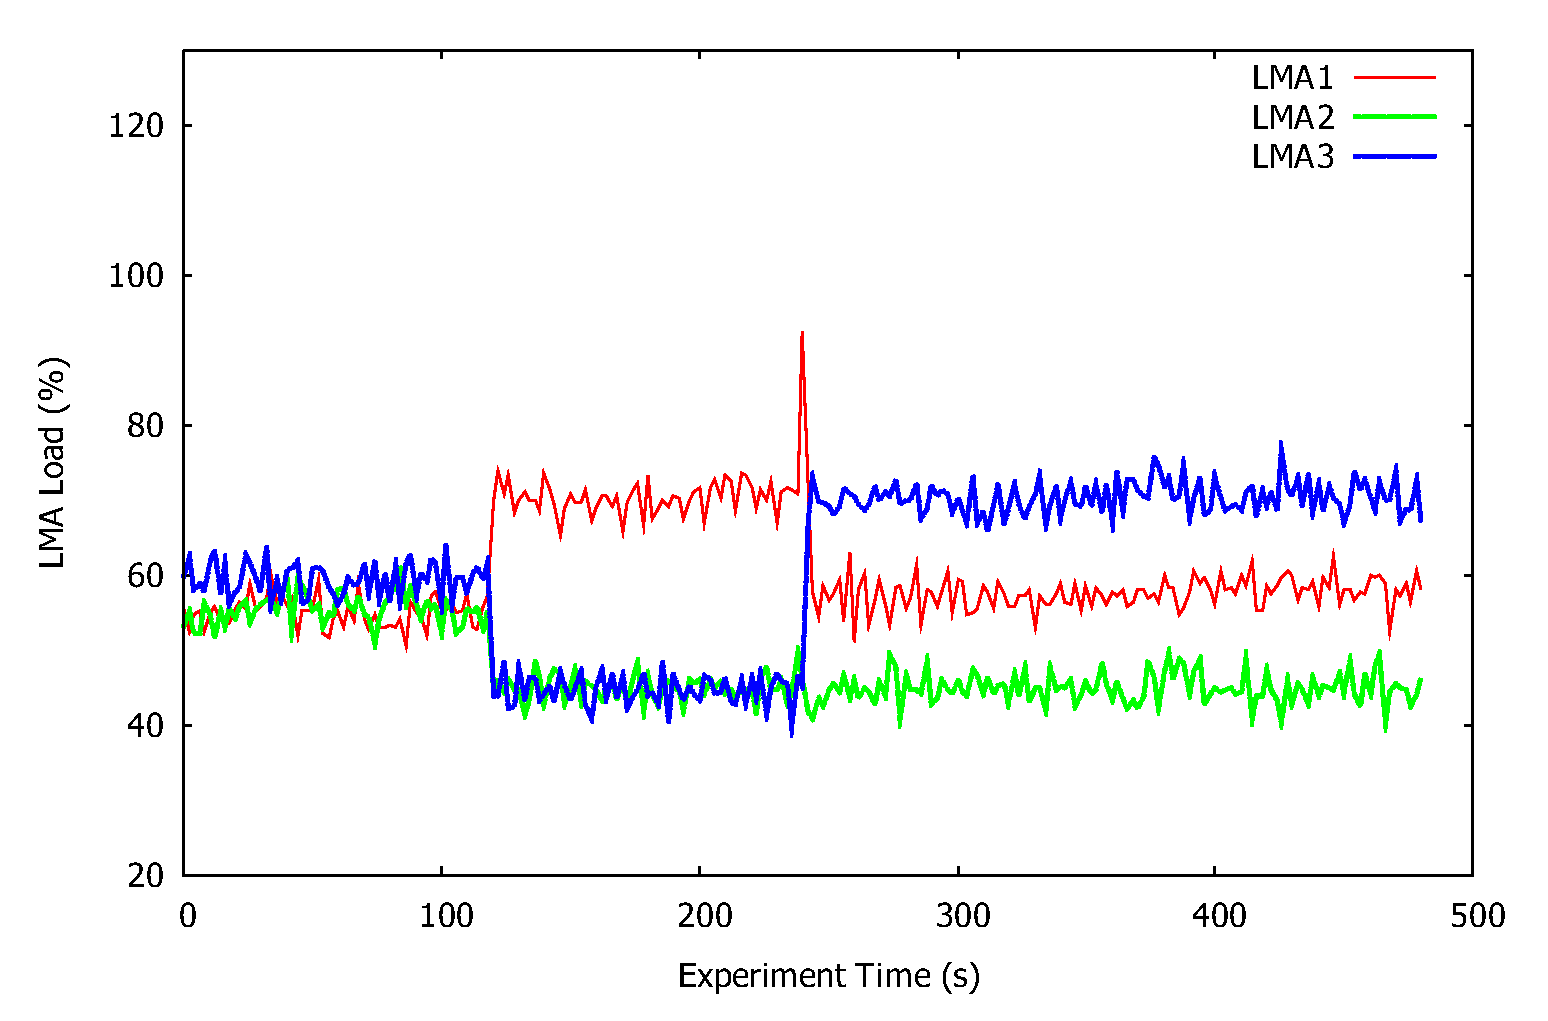
\includegraphics[width=0.35\textwidth]{./Part2/Chapter5/figures/reactive_multicast_result.eps}\label{fig:s2_reactive_multicast}}
\caption[LMA load in the experimentation.]{LMA load in the scenario 2 (experiment 2): (a) pure-PMIP , b) reactive-MN approach, (b) reactive-multicast approach.}
\label{fig:scenario2}
\end{figure}
The detail of load distribution of different approaches is plotted in Fig.~\ref{fig:scenario2}. The reactive-multicast helps avoid $LMA_{1}$ from being overloaded. Meanwhile, the overload status cannot be resolved in the reactive-MN approach ($LMA_{1}$ is still overloaded, while $LMA_{13}$ load is greatly increased). As a result, the total load of all LMAs is significantly increased compared to that in the pure-PMIP and reactive-multicast approach. It is due to the fact that the $LMA_{3}$ has to join the channel $C_{12}$ while $LMA_{1}$ continues forwarding this channel. In this case, more than 31\% of the LMA capacity is wasted. 
\subsection{Multicast Service Disruption Time}
In this subsection, the following parameter values are used: $t_{mm}$ = $t_{ll}$ 
= $t_{la}$ = $t_{rr}$ = 10 ms, $t_{ml}$ = $t_{mc}$ =20 ms, $t_{wl}$=15 ms, $t_{join}$ =13.5 ms, $D_{L2}$ = 50 ms, and $t_{qrd}$ = 374.2 ms. $t_{cv}$ is typically in seconds (for example, the default value in case of OSPF is 10 seconds) \cite{ospf_convergence,ospf_timer}. In this subsection, it is set to 1s. The value of $n_{mr}$ is varied over a range [0, 10] hops. It is noted that most parameters used in this evaluation are set to the typical values found in \cite{Thinh_WCNC_Multicast} and \cite{dsrm}. 

\begin{figure}[h!]
\centering
\subfloat[]{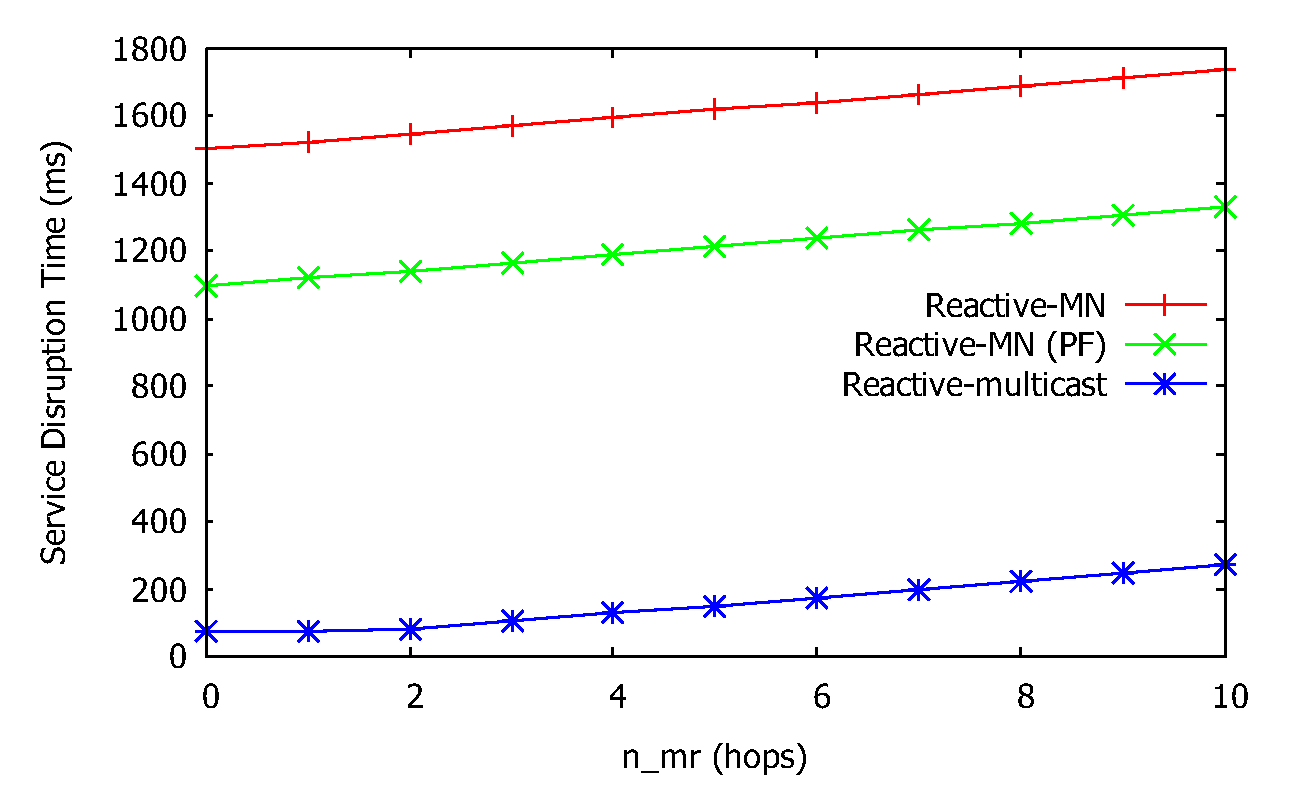
\includegraphics[width=0.47\textwidth]{./Part2/Chapter5/figures/c7_sd_n_mr.eps} \label{fig:service_disruption}}\,\,\,\,\,\,
\subfloat[]{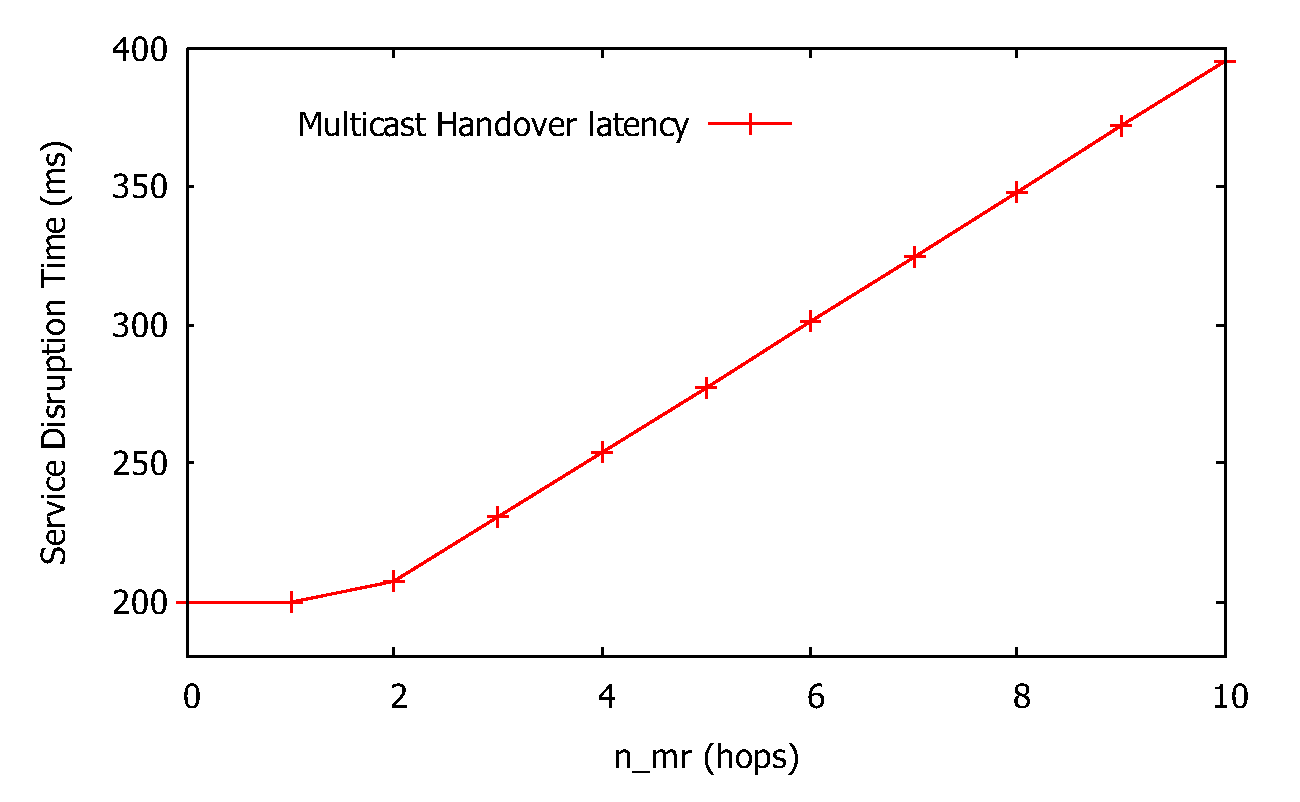
\includegraphics[width=0.47\textwidth]{./Part2/Chapter5/figures/c7_ho.eps}\label{fig:service_disruption_HO}}
\caption[Service disruption time as a function of the average hop-count distances.]{Service disruption time as a function of $n_{mr}$: (a) caused by LB mechanisms, (b) by handover.}
\label{fig:sd}
\end{figure}

Fig.~\ref{fig:service_disruption} shows the multicast service disruption time as a function of $n_{mr}$. It appears clearly that the service disruption in the reactive-MN ($D_{R\_MN}$ and $D_{R\_MN\_PF}$) is definitely higher than the maximum tolerant interruption time for normal services, as specified in \cite{interruption_requirements} is 500ms. Thus, it causes a noticeable service disruption. On the other hand, the service disruption in the reactive-multicast is kept below the value of 300ms, thus, satisfying the requirements for the real-time services. In other words, the reactive-multicast approach helps greatly reduce the service disruption compared to the reactive-MN solution. Moreover, in the reactive-multicast approach, if there exist the LMA which already had the forwarding state for this channel and is not overloaded, it should be chosen as the tLMA. As a result, it is high probably that the $d_{join}$ and $d_{deliver}$ are ignored. That means in most cases $D_{R\_M}$ is 75 ms. 

Fig.~\ref{fig:service_disruption_HO} shows the service disruption time during handover as a function of $n_{mr}$. We could observe that when $n_{mr}<6$, the handover latency is below the value of 300 ms. Moreover, in most cases the multicast traffic is already available at the tLMA, thus, the service disruption during handover is 200 ms. Consequently, the handover impact on the quality of multicast flow is almost imperceptible.
\section{Conclusion} \label{ch7:conclusion}
As the multicast is expected to be widely used in the future networks, degrading the role of the multicast in the available LB mechanism can cause some issues not only from LB perspective (degradation of efficiency) but also from multicast perspective (tunnel convergence problem and service disruption).  To overcome these issues, a multicast-based solution has been proposed. The benefit of the solution is that it does not influence the other ongoing unicast/multicast sessions. It can also co-operate with the existing LB proposals to improve the performance of the network.

Via a near-to-real testbed, the experiment results show that the proposed solution helps better distribute the load imposed by the multicast service among LMAs. Additionally, it helps greatly reduce the multicast service disruption time caused by a changed LMA for LB purpose compared to the existing proposals, even satisfying the service disruption requirement for the real-time services.  

However, from the performance analysis and the experiment result, we conclude that none of the two solutions is complete. The multicast-based solution in general works well in the domain where the mobile data traffic is dominated by the multicast traffic; the unicast-based solution, in contrast, works well with the unicast-dominated domain. For instance, the multicast-based solution may be the most convenient for distributing load among the multicast tree mobility anchors (MTMA) which work as a topological anchor point for the multicast traffic in a PMIPv6 domain \cite{ro_pmip}. It comes from the fact that the MTMA only serves the multicast traffic. As a result, the multicast-based should co-operate with the MN-based solution to enhance the reliability and scalability of  the network. For example, the proactive-MN can be applied when an MN enters the PMIPv6 domain, while the proactive-multicast is evolved when a multicast session is initiated. Besides, the reactive-multicast can be followed by the reactive-MN approach. At this stage, if any multicast session is not a real-time and delay sensitive one, the reactive-multicast approach will be performed. Otherwise, the reactive-MN will be executed. The main idea is that we try to distribute load among LMAs by using the multicast-based solution before applying the reactive-MN solution to avoid the influence on the ongoing sessions. Therefore, the blocking probability of a new MN (session) and the dropping probability of the existing MNs (sessions) are obviously lower than the existing LB mechanisms (lower is better).




